\documentclass[12pt,a4paper,notitlepage]{article}
\usepackage[utf8]{inputenc}
\usepackage[english]{babel}
\usepackage[T1]{fontenc}
\usepackage[affil-it]{authblk}
\usepackage[backend=biber,
			style=authoryear-icomp,
			sortlocale=de_DE,
			natbib=true,
			isbn=false,
			doi=false,
			bibstyle=authoryear,
			]{biblatex}
\usepackage{eurosym}
\usepackage{enumitem}
\usepackage{url}
\usepackage{blindtext}
\usepackage{hyperref}
\usepackage{breakurl}
\usepackage{amsmath}
\usepackage{titling}
\usepackage{amsfonts}
\usepackage{amssymb}
\usepackage{pgfplots}
\usepackage{caption}
\usepackage{subcaption}
\usepackage{graphicx}
\usepackage{dcolumn}
\usepackage{tikz-3dplot}
\usepackage{subcaption}
\usepackage{float}
\usepackage{adjustbox}
\usepackage{multirow,rotating}
\usepackage[autostyle]{csquotes}
\usepackage[toc,page]{appendix}
\usepackage{lscape}
\usepackage{todonotes}
\usepackage{booktabs}
\usepackage{multirow}
\usepackage{bm}
\usepackage{eurosym}
\usepackage{pdflscape}
\usepackage{geometry}
\geometry{a4paper,left=30mm,right=20mm, top=2cm, bottom=2cm} 

\addbibresource{Textmining.bib}
\ExecuteBibliographyOptions{maxcitenames=2,mincitenames=1}
\renewcommand*{\mkbibnamelast}[1]{\textsc{#1}}

\title{Matching agendas}
\date{\today}

\author{Franziska Löw
  \thanks{Electronic address: \texttt{loewf@hsu-hh.de}}}
\affil{Department of Industrial Economics,\\ Helmut Schmidt University,\\ Hamburg, Germany}

\begin{document}
\begin{titlepage}
	\maketitle
	\begin{abstract}
	To measure the political slant of german online newspaper the topics addressed in newspapers are compared with topics addressed in press releases of political parties. To find the latent topics in the corpus a structural topic model is conducted. 

	\end{abstract}

\end{titlepage}

\tableofcontents

\pagebreak

%------------------------------------------------%
%----------------- Begin paper -------------------%
%------------------------------------------------%

\section{Introduction}

In recent years, the media and their role in the perception and decision of individuals in the political context have been increasingly subject to criticism. Terms such as "fake news" or "quality journalism" are currently part of almost every debate regarding the role of the media. Critics accuse the media of reporting biased on certain parties or political events and thus influencing the political consciousness of voters. This raises the unavoidable question of what biased reporting actually means or, on the contrary, what objective reporting is and if this is even possible. A journalist who writes an article about a certain topic puts rough facts (e.g. figures on economic indicators) into a context, such that each article is shaped by the subjectivity of this journalist. Similarly, an editor of a media outlet has to select the topics to be discussed in the medium from a large pool of reports. Thus, to a certain extent, media is always filtered by journalists' perceptions and editorial decisions. 

A legitimate question, however, could be which factors or incentives lead to the selection or deselection of certain topics. On the one hand, one could assume that editors select the topics and articles that correspond to their own political views. A profit-maximizing editor, on the other hand, would tend to adapt the selection to readers' preferences. (Some populist voices would even claim that - at least the so called "mainstream media" - is controlled by the government.) 

In order to answer these and other media-related questions in the political context, quantifying the content of media is essential. In other words, what features can be used to measure the content of, for example, an online article? The literature of communication science, for example, often uses visibility (how often political actors appear in the media) or tonality (how they are evaluated) in this regard. In addition to these actor-based approaches, there are also more issue-based approaches to be found in communication science as well as in other disciplines. In this case, the contents or the language used by media are compared with the contents or the language used by political actors in order to identify whether political actors are able to place their own policy positions in the media using their own language. Leading studies from economic literature, for example, examine how often a newspaper quotes the same think tanks \citep{groseclose_measure_2005, lott_is_2014} or uses the same language \citep{gentzkow_media_2004} as members of Congress. 

To measure the ideological content of several online news services in Germany, in the present paper I compare the topics discussed in these media with the press releases of the parties in the german "Bundestag" using a structural topic model (STM) developed by \citet{roberts_model_2016}. The dataset contains nearly 12.000 online news articles from seven major news provider dated from June 1, 2017 to March 1, 2018 as well as over 1.900 press releases of the parties in the german "Bundestag". As the German federal elections took place on 24th of September 2017 and the formation of the government has taken up a period of about five months, the articles considered inform their readers about both the election promises of the parties (before the election) and the coalition talks (after the election). To discover the latent topics in the corpus of text data, the structural topic model (STM) developed by \citet{roberts_model_2016} is applied. The STM is an unsupervised machine learning approach that models topics as multinomial distributions of words and documents (as a synonym for news articles) as multinomial distributions of topics, allowing the incorporation of external variables that affect both, topical content and topical prevalence. The results of the generative process of the STM are two posterior distributions: One for the topic prevalence in a document (what is the article or press release about?) and one for the content of a topic (what is the topic about?). In the next step the topics addressed in campaign communication (i.e., the party agenda) are compared with the topics the parties address in media coverage (i.e., the mediated party agenda). The results of this analysis are then compared with data on the political orientation of consumers in order to evaluate whether there may be a link between consumer preferences and the slant-index of a medium. 

The use of online news as data input accurately reflects the changed conditions in the news market as the importance of the internet as a source of information for political topics has grown strongly in recent years.\footnote{Even though television remains the most widely used source of news in Germany (2018: 74\%), numbers watching continue to decline while use of the internet for news has grown significantly in the last year (+5\%, 2018: 65\%) \citep{holig_reuters_2018}.} This trend has as strong effect on the market for media content as neither supply nor demand is tied to specific times and can adapt to events in real time. Users can consume their preferred news sources at any time and providers can adapt their offerings to events in real time without waiting for the next issue or TV show.

The research contribution of this paper is twofold: First, a new method for the calculation of the slant-index is presented that allows an extensive content analyses of newspaper coverage and party press releases and at the same time reduces human induced bias and makes research more traceable and comparable. In addition, a new dataset of online news is used, which has a significant relation to the current discussion of the media in the political context. 

The remaining course of the paper is as follows: The following section provides an overview of the related literature. Section \ref{ch_elections} gives an introduction to the political trends within the considered time (June 2017 to March 2018). The data used to conduct the model is described in section \ref{ch_data}. Section \ref{ch_generativeProcess} explains the generative process of the structural topic model as well as the selected parameters to run the model. The empirical analysis is conducted in section \ref{ch_regression}. 

%-------------------------------------------------------%
%----------------- Literature Review -------------------%
%-------------------------------------------------------%

\section{Literature}

In unbiased media reporting all political sides should be equally represented according to some kind of benchmark for balance or neutrality \citep{hopmann_political_2012}. Bias is then defined as the extent to which media reporting deviates from this benchmark.

However, the discussion about media bias has not only been studied since the growing importance of the internet. Different research disciplines investigate the concept of media bias, albeit with different focus. Regardless of the discipline, media bias research can be roughly divided into three research questions: (1) What types of bias exist, (2) how and why does it emerge and (3) what influence does it have on the political outcomes. While 1 and 3 are dealt with in economic, political and communication research, question 2 is mainly addressed in economic literature. It investigates which forces on the supply and demand side drives to media bias.  

%---- economic literature --- %
The general hypothesis within economic literature is that (1) different media outlets tend to report "biased" or "slanted" \citep{groseclose_measure_2005, lott_is_2014} and (2) that media reporting about political news may have a profound influence on political outcomes \citep{gentzkow_media_2004, stromberg_radios_2004, dellavigna_fox_2006, snyder_press_2010, gentzkow_television_2006}. 

In the economic literature the market dynamics that lead to a possible bias are analysed. In principle, media bias can come from the supply side, and reflect the preferences of journalists \citep{baron_persistent_2006}, editors, or owners (Besley and Prat, 2004). Alternatively, media bias can come from the demand side, and reflect the news providers' profit-maximizing choice to cater to the preferences of the consumers. 

%---- communication research ---%

 While economic research investigates the market dynamics that lead to media bias, communication science is more concerned with the question of what different types of bias exist. According to a \citet{dalessio_media_2000} the concept of media bias actually encompasses different subtypes: (1) Coverage bias, (2) tonality bias und (3) agenda bias. These three concepts measure how often political actors appear in the media (coverage bias), how they are evaluated (tonality bias) and whether they are able to present their own political positions and talk about their issues in the media (agenda bias).
 
% ---- visibility bias ----
There is visibility bias when a party is the subject of an undue amount of coverage compared to the benchmark of that party at a given point in time. Media that reports biased in that sense influences voters behaviour in such way, that voters tend to prefer parties that are more visible in their media repertoire \citep{eberl_one_2017}. Studies combining media content data with voter surveys have indeed found that the mere visibility of parties and candidates is an important factor influencing vote choice (Oegema & Kleinnijenhuis, 2000). The amount of a parties campaign communication or their standing in polls are commonly used as a reference point \citep{junque_de_fortuny_media_2012, hopmann_political_2012}. 

\citet{eberl_one_2017} use the average visibility of all parties in each media outlet during the period of their analysis as a key benchmark to capture whether party visibility is biased in comparison to what is typical for that outlet and are therefore able to compare party visibility between outlets. Applying a similar logic to tonality and agenda bias, they measure the effect of the different bias on user voting behaviour using an online panel survey from the Austrian parliamentary election campaign of 2013. 


% ---- tonality bias ----

- \citet{druckman_impact_2005} argue that the audience's conclusions about parties are automatically drawn from positive or negative descriptions in texts about the parties. 

- Similarly, valence framing suggests that public awareness of parties is affected depending on whether they are highlighted with positive or negative aspects in the media \citep{de_vreese_valenced_2006, hurtikova_importance_2017}.  

To measure tonality in a text, studies differ between manually coded data (e.g. \citet{eberl_one_2017}) and dictionary-based analysis ( e.g. \citep{junque_de_fortuny_media_2012}). The latter approach is widely used outside the area of media content analysis. To conduct such an analysis, a lists of words (dictionary) associated with a given emotion, such as negativity is pre-defined by the analyst. The document is then deconstructed into individual words and the frequencies of words contained in a given dictionary are calculated. Such lexical or "bag-of-words"€ approaches are widely presented in the finance literature to determine the effect of central banks' monetary policy communications on asset prices and real variables (\citet{nyman_news_2018} \citet{tetlock_giving_2007}, \citet{tetlock_more_2008}). \citet{hansen_shocking_2016} use a similar approach to explore the effects of FOMC (Federal Open Market Committee) statements on both market and real economic variables. To calculate their score, they subtract the negative words from the positive words und divide this by the number of total words of the statement. A similar score is used by \citet{nyman_news_2018}, who measure the effect of narratives and sentiment of financial market text-based data on developments in the financial system. 

In the domain of media content analysis \citet{junque_de_fortuny_media_2012} count the sentiment words in a window of two sentences before and after the mention of a political party and assuming uniformity of sentiment distribution among parties to measure the bias.\footnote{A similar approach for target identification with a 10-word window is used in \citet{balahur_sentiment_2013}} They use a text-mining approach to automate the analysis of a large text corpus showing techniques to measure both visibility and tonality bias. The former is benchmarked by the amount of preference votes for that party. Similar to \citet{junque_de_fortuny_media_2012} the present study uses techniques that allow the computational analysis of a large dataset of text-data. However, a different reference point is used to allow for a comparison between media outlets. Additionally, agenda bias is measured based on the comparison between the content of online news and parties press releases \citet{eberl_one_2017}.  

% ---- agenda bias ----
Overall, most research tends to disregard agenda bias as the operationalization is more challenging. In order to know which news stories have been held out by journalists, the true universe of news stories at a given point in time has to be known \citet{dalessio_media_2000}. However, a greater dissemination of a party's political content may have a positive impact on attitudes towards that party \citep{benewick_floating_1969, eberl_one_2017}. \citet{brandenburg_party_2006} measure partisan tendencies in reporting in terms of all three biases. Utilizing content analysis data from the 2005 General Election campaign they show that increasingly ambiguous endorsements translate into an absence of open support for political parties. Similarly, \citet{eberl_one_2017} find that voters evaluate parties more favorably if those parties addressed their own favored topics more prominently in media coverage. In their analysis media content was analyzed using manual content analysis of political claims on a sentence level.

What drives media bias?
In principle, media bias can come from the supply side, and reflect the preferences of journalists \citep{baron_persistent_2006}, editors, or owners (Besley and Prat, 2004). Alternatively, media bias can come from the demand side, and reflect the news providers' profit-maximizing choice to cater to the preferences of the consumers.

% -----  STM --------
The STM developed by \citet{roberts_model_2016} is a recent extension of the standard topic modelling technique, labeled as latent Dirichlet allocation (LDA), which refers to the Bayesian model in \citet{blei_latent_2003} that treats each word in a topic and each topic in a document as generated from a Dirichlet - distributed prior.\footnote{See also \citet{griffiths_probabilistic_2002}, \citet{griffiths_finding_2004} and \citet{hofmann_probabilistic_1999}. \citet{pritchard_inference_2000} introduced the same model in genetics for factorizing gene expression as a function of latent populations.} Since its introduction into text analysis, LDA has become hugely popular and especially useful in political science.\footnote{see \citet{blei_probabilistic_2012}, \citet{grimmer_text_2013} and \citet{wiedmann_text_2016} for an overview in social science and \citet{gentzkow_text_2017} give an overview of text mining applications in economics.} \citet{wiedmann_text_2016} uses topic model methods on large amounts of news articles from two german newspapers published between 1959 and 2011, to reveal how democratic demarcation was performed in Germany over the past six decades. \citet{paul_cross-collection_2009} compares editorial differences between media sources, using cross-collection latent Dirichlet allocation (ccLDA), an LDA-based approach that incorporates differences in document metadata. They use a dataset of 623 news articles from August 2008 from two American media outlets - msnbc.com and foxnews.com - to compare how they discuss topics. Reviewing the top words of the word-topic distribution, they find some content differences between the two media sources under review. 

The difference between the widely used LDA and the STM approaches lies in how $\theta$ and $\phi$ are determined. LDA assumes that $\theta ~ \text{Dirichlet}(\alpha)$ and $\phi ~ \text{Dirichlet}(\beta)$, where $\alpha$ and $\beta$ are fitted with the model. While for STM, the prior distributions for $\theta$ and $\phi$ depend on document-level covariates (e.g. the author or date of a document). For this purpose, the the STM specifies two design matrices of covariates, where each line defines a vector of covariates for a specific document.  In $X$, the covariates for topic prevalence are given, so that the probability of a topic for each document varies according to X, rather than resulting from a single common prior. The same applies to $Z$, in which the covariates for the word distribution within a topic are specified. 

The model has been applied to multiple academic fields: \citet{roberts_structural_2014} uses STM to analyze open-ended responses from surveys and experiments, \citet{farrell_corporate_2016} applies the model to scientific texts on climate change, revealing links between corporate funding and the framing of scientific studies. \citet{mishler_using_2015} show that "STM can be used to detect significant events such as the downing of Malaysia Air Flight 17" when applied to twitter data. Another study shows how STM can be used to explore the main international development topics of countries'€™ annual statements in the UN General Debate and examine the country-specific drivers of international development rhetoric \citep{baturo_what_2017}. \citet{mueller_reading_2016} use newspaper text to predict armed conflicts in different regions. They use the estimated topic shares in linear fixed effects regression to forecast conflict out-of-sample. \citet{roberts_navigating_2016} use STM to examine the role of partisanship in topical coverage using a corpus of 13,246 posts that were written for 6 political blogs during the course of the 2008 U.S. presidential election. With the aim of revealing the effect of partisan membership on topic prevalence, each blog is assigned to be either liberal or conservative. To explore the differences between the two, they look at the expected proportion of topics and examine the posts most associated with a respective topic. This approach is similar to \citet{roberts_model_2016}. 

The present analysis differs from earlier approaches to measure agenda bias in that a machine learning technique is used to identify the underlying topics in the text corpus applying a structural topic model \citep{roberts_model_2016}. Furthermore, I use text-mining techniques to measure coverage and tonality bias. However, I shall refrain as far as possible from interpreting the results at political level. Rather, it is my goal to show how text mining techniques enable an efficient and objective analysis of today's online media landscape and simultaneously allow the analysis to be reproduced. 

% ---------------------
% Backup from FE regression
% ----------------------

Much of the research on online content and political trends have focused on traditional weblogs and social media websites, such as Twitter, Facebook, MySpace, and YouTube. These studies have shown that social media is used to spread political opinions and that these considerations reflect the political landscape of the offline world. \citet{tumasjan_predicting_2010} investigate Tweets between August 13th and September 19th, 2009, prior to the German national elections to examine whether Twitter messages reflect the current offline political sentiment and whether it can be used to predict the popularity of parties or coalitions in the real world. With regard to the later question, they compare the share of attention the political parties receive on Twitter with the election result to examine whether the activity on Twitter can serve as a predictor of the election outcome. They found that the number of tweets reflects the election result and even comes close to traditional election polls.

\citet{fu_analyzing_2013} use a corpus of online posts from discussion forums and blogs to examine the extent to which online sentiment reflected in social media content can predict phone survey results in Hong Kong. They build a sentiment classifier conducting a support vector machine analysis on a training set of 2,000 manually labeled posts. In order to evaluate the temporal relationship between the time series of the online sentiment score and the results of the telephone survey, a cross correlation analysis was conducted, using the Box and Jenkins autoregressive integrated moving average (ARIMA) method \citep{box_time_2008}. Estimating the cross-correlation functions of the residuals, they find that online sentiment scores can lead phone survey results by about 8–15 days. 

In a more recent conference paper, \citet{padmaja_evaluating_2014} identify the scope of negation in news articles for two political parties in India (BJP and UPA) to analyze how the choice of certain words used in these texts influence the sentiments of public in polls. Comparing three different sentiment analysis methods (two machine learning and one dictionary method), they observe that the choice of certain words used in political text was influencing the sentiments in favor of BJP. They conclude that this sentiment bias might be one of the causes for the election results in 2014.

\citet{dewenter_can_2018} use human-coded data from leading media in Germany together with the German Politbarometer survey to investigate how media coverage affects short- and long-term political preferences between February 1998 and December 2012. They find a positive correlation between the media coverage and the short-term voting intention for a political party. In the long-term, however, voting preferences are stable. 
 
% -------------------------
% Background Bundestagswahl
% -------------------------
\section{Background on the federal election in Germany (2017)}\label{ch_elections}

The articles analyzed in this paper cover a period from June 1, 2017 to March 1, 2018 and thus cover both the most important election campaign topics for the Bundestag elections on September 24, 2017 and the process of forming a government that lasted until February 2018. After four years in a grand coalition with the Social Democrats (SPD), German Chancellor Angela Merkel, member of the conservative party CDU/CSU (also known as Union), ran for re-election. The SPD nominated Martin Schulz as their candidate. 

On the right side of the political spectrum, AfD (alternative for Germany) managed to be elected to the German Bundestag for the first time in 2017. The political debate about the high refugee numbers of the past years brought a political upswing to the AfD, which used the dissatisfaction of parts of the population to raise its own profile. In the course of the reporting on the federal elections, leading party members of the AfD as well as party supporters repeatedly accused the mass media of reporting unilaterally and intentionally presenting the AfD badly.

After the election, the formation of a government was difficult due to the large number of parties elected to the Bundestag and the considerable loss of votes by the major parties CDU/CSU and SPD. Since all parties rejected a coalition with the AfD, numerically only two coalitions with an absolute parliamentary majority were possible: a grand coalition ("GroKo" - from the German word Groߟe Koalition) of CDU/CSU and SPD, and a Jamaica coalition (coalition of CDU/CSU, FDP (economic liberal party) and B90/Die Grünen (Bündnis 90/Die Grünen, green party)). The grand coalition was initially rejected by the SPD. The four-week exploratory talks on the possible formation of a Jamaica coalition officially failed on November 19, 2017 after the FDP announced its withdrawal from the negotiations. FDP party leader Christian Lindner said that there had been no trust between the parties during the negotiations. The main points of contention were climate and refugee policy. CDU and CSU regretted this result, while B90/Die Grünen sharply criticized the liberals'€™ withdrawal. The then Green leader Cem Özdemir accused the FDP of lacking the will to reach an agreement.

After the failure of the Jamaica coalition talks, a possible re-election or a minority government as alternatives were discussed in the media before the SPD decided to hold coalition talks with the CDU/CSU. This led to great resistance from the party base, which called for a party-internal referendum on a grand coalition. After the party members voted in favor of the grand coalition, a government was formed 171 days after the federal elections. 

Figure \ref{fig_polls} shows that support for the two major popular parties has been declining in recent months since August 2017, with the CDU/CSU again showing positive survey results since November 2017.\footnote{For each party the survey results of the seven major institutes are considered. To calculate a smooth line for each party on each day, the moving average within 15 days (7 before the day, 7 after the day, and the day itself) is estimated. The data source is [wahlrecht.de](https://www.wahlrecht.de/).} However, the poll results of the SPD have been falling since March 2017. At the same time, the AfD in particular has been recording increasingly positive survey results since June 2017.  

\begin{figure}[H]
\begin{center}
	\caption{Election Polls}
	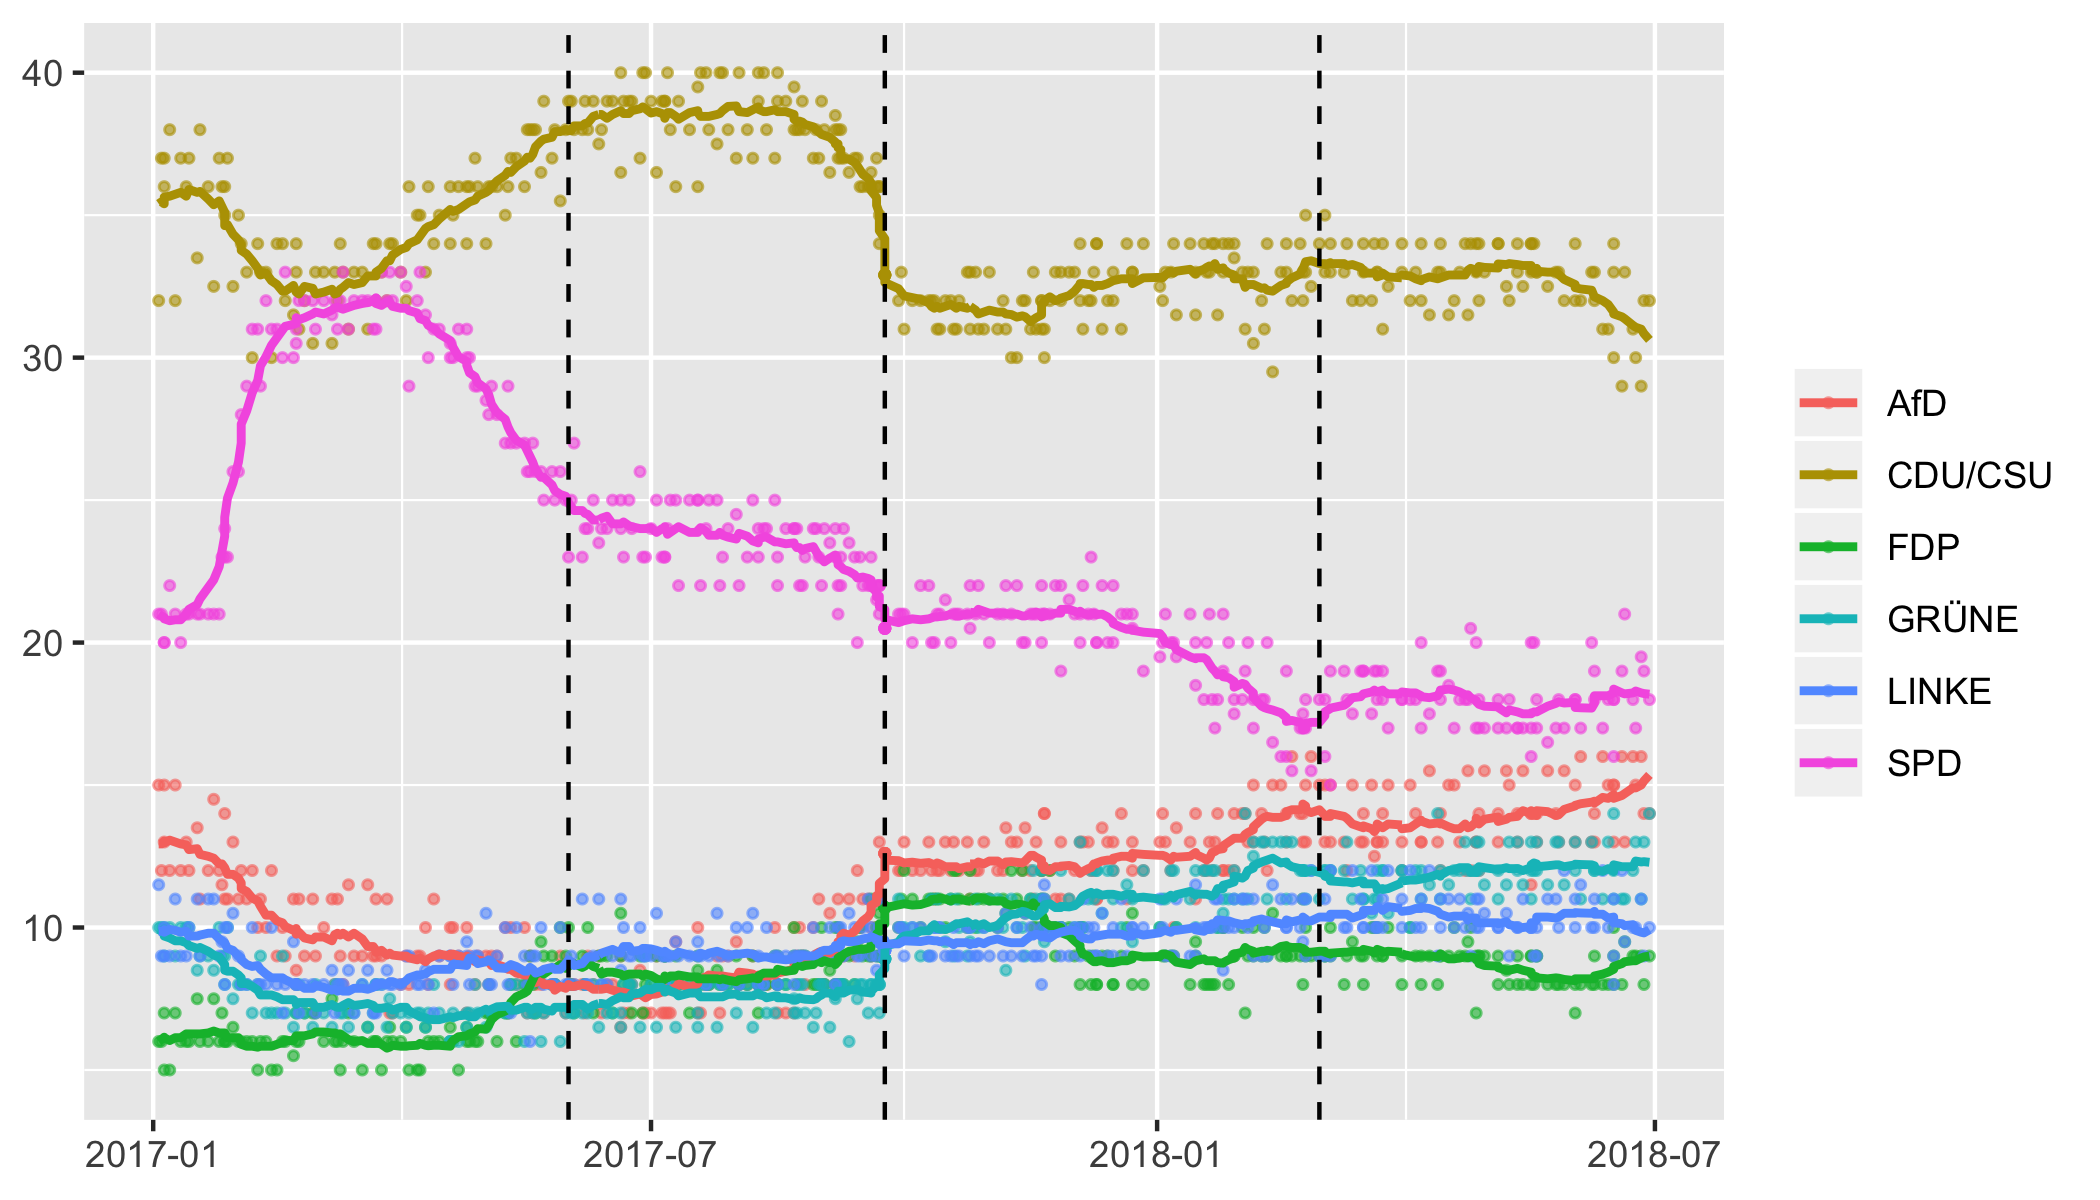
\includegraphics[width=0.9\textwidth]{../figs/polldata}
	\label{fig_polls}
	\end{center}
\end{figure}

% -------
% Method
% -------
\section{Measuring slant-index}\label{ch_method}
 
My approach to measuring the slant of a newspaper is to compare the topics in the newspaper with topics in parties' press releases to identify which parties the topics in the newspaper are most similar to. Parties want the media agenda to be congruent with their own agenda to define the issue-based criteria on which they will be evaluated by voters \citep{eberl_one_2017}. Thus, parties instrumentalize their press releases in order to highlight issues that they are perceived to be competent on, that they "own" and that are important to their voters \citep{kepplinger_einfluss_2004}. Editors can select from this universe and decide which topics will be discussed in the news. In that sense the ideological content of a newspaper refers to the extent to which the topics promoted by the parties correlate with the topics discussed in the news articles.

To discover the latent topics in the corpus of press releases (1.942) and news articles (11.880), a structural topic modeling (STM) developed by \citet{roberts_model_2016} is applied. The STM is an unsupervised machine learning approach that models topics as multinomial distributions of words and documents as multinomial distributions of topics, allowing to incorporate external variables that effect both, topical content and topical prevalence. The results of the generative process of the STM are two posterior distributions: One for the topic prevalence in a document (what is the article or press release about?) and one for the content of a topic (what is the topic about?). Subsequently the bivariate correlations between party agendas and the mediated party agendas in the online news are estimated. These correlations represent the agenda selectivity each party experiences in each media outlet. The higher the correlation, the more congruent both agendas are. 

This section first describes the data on news articles and press releases and how they have processed in order to use them as input for the model.

% -----
% Data
% -----
\subsection{Data}\label{ch_data}

\subsubsection{Press releases}

Press releases published by parties and those published by the parliamentary groups (or factions) in the Bundestag should be considered in different ways as parties are financed by membership dues, donations and campaign expenses, while factions are financed by state funds. According to Parteigesetzt §25 (2) state funded factions may not support partie, as there would be a disadvantaged for parties that are not in the Bundestag. However, since it is difficult to draw the line between faction activity and election campaign assistance, I assume that factions intervene in the public perception of this party with their press releases, which is why I include both the press releases of the federal party and the federal faction \citep{kepplinger_einfluss_2004}.

\begin{figure}[H]
\begin{center}
	\caption{Press releases}
	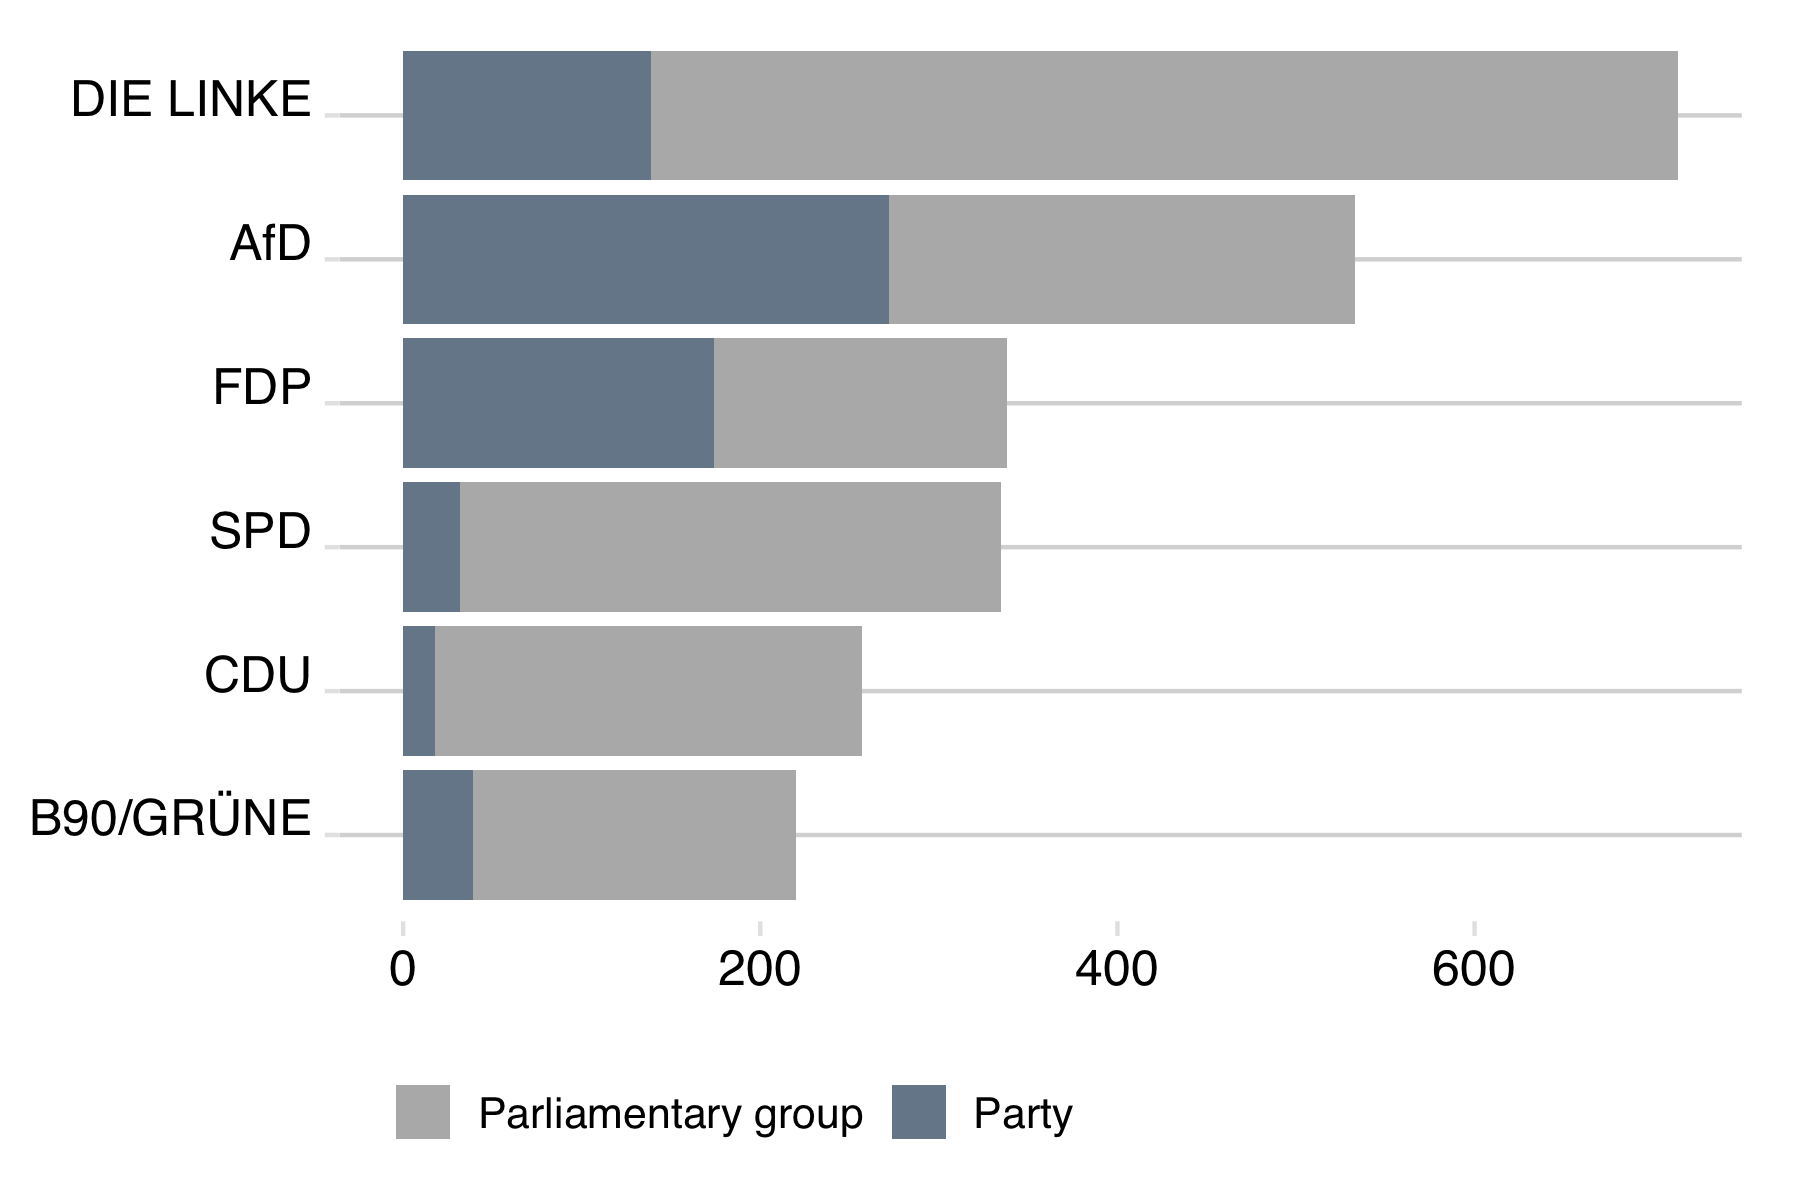
\includegraphics[width=0.7\textwidth]{../figs/press_releases}
	\label{fig_press}
	\end{center}
\end{figure}

After pre-processing

\begin{figure}[H]
\begin{center}
	\caption{Term-frequency}
	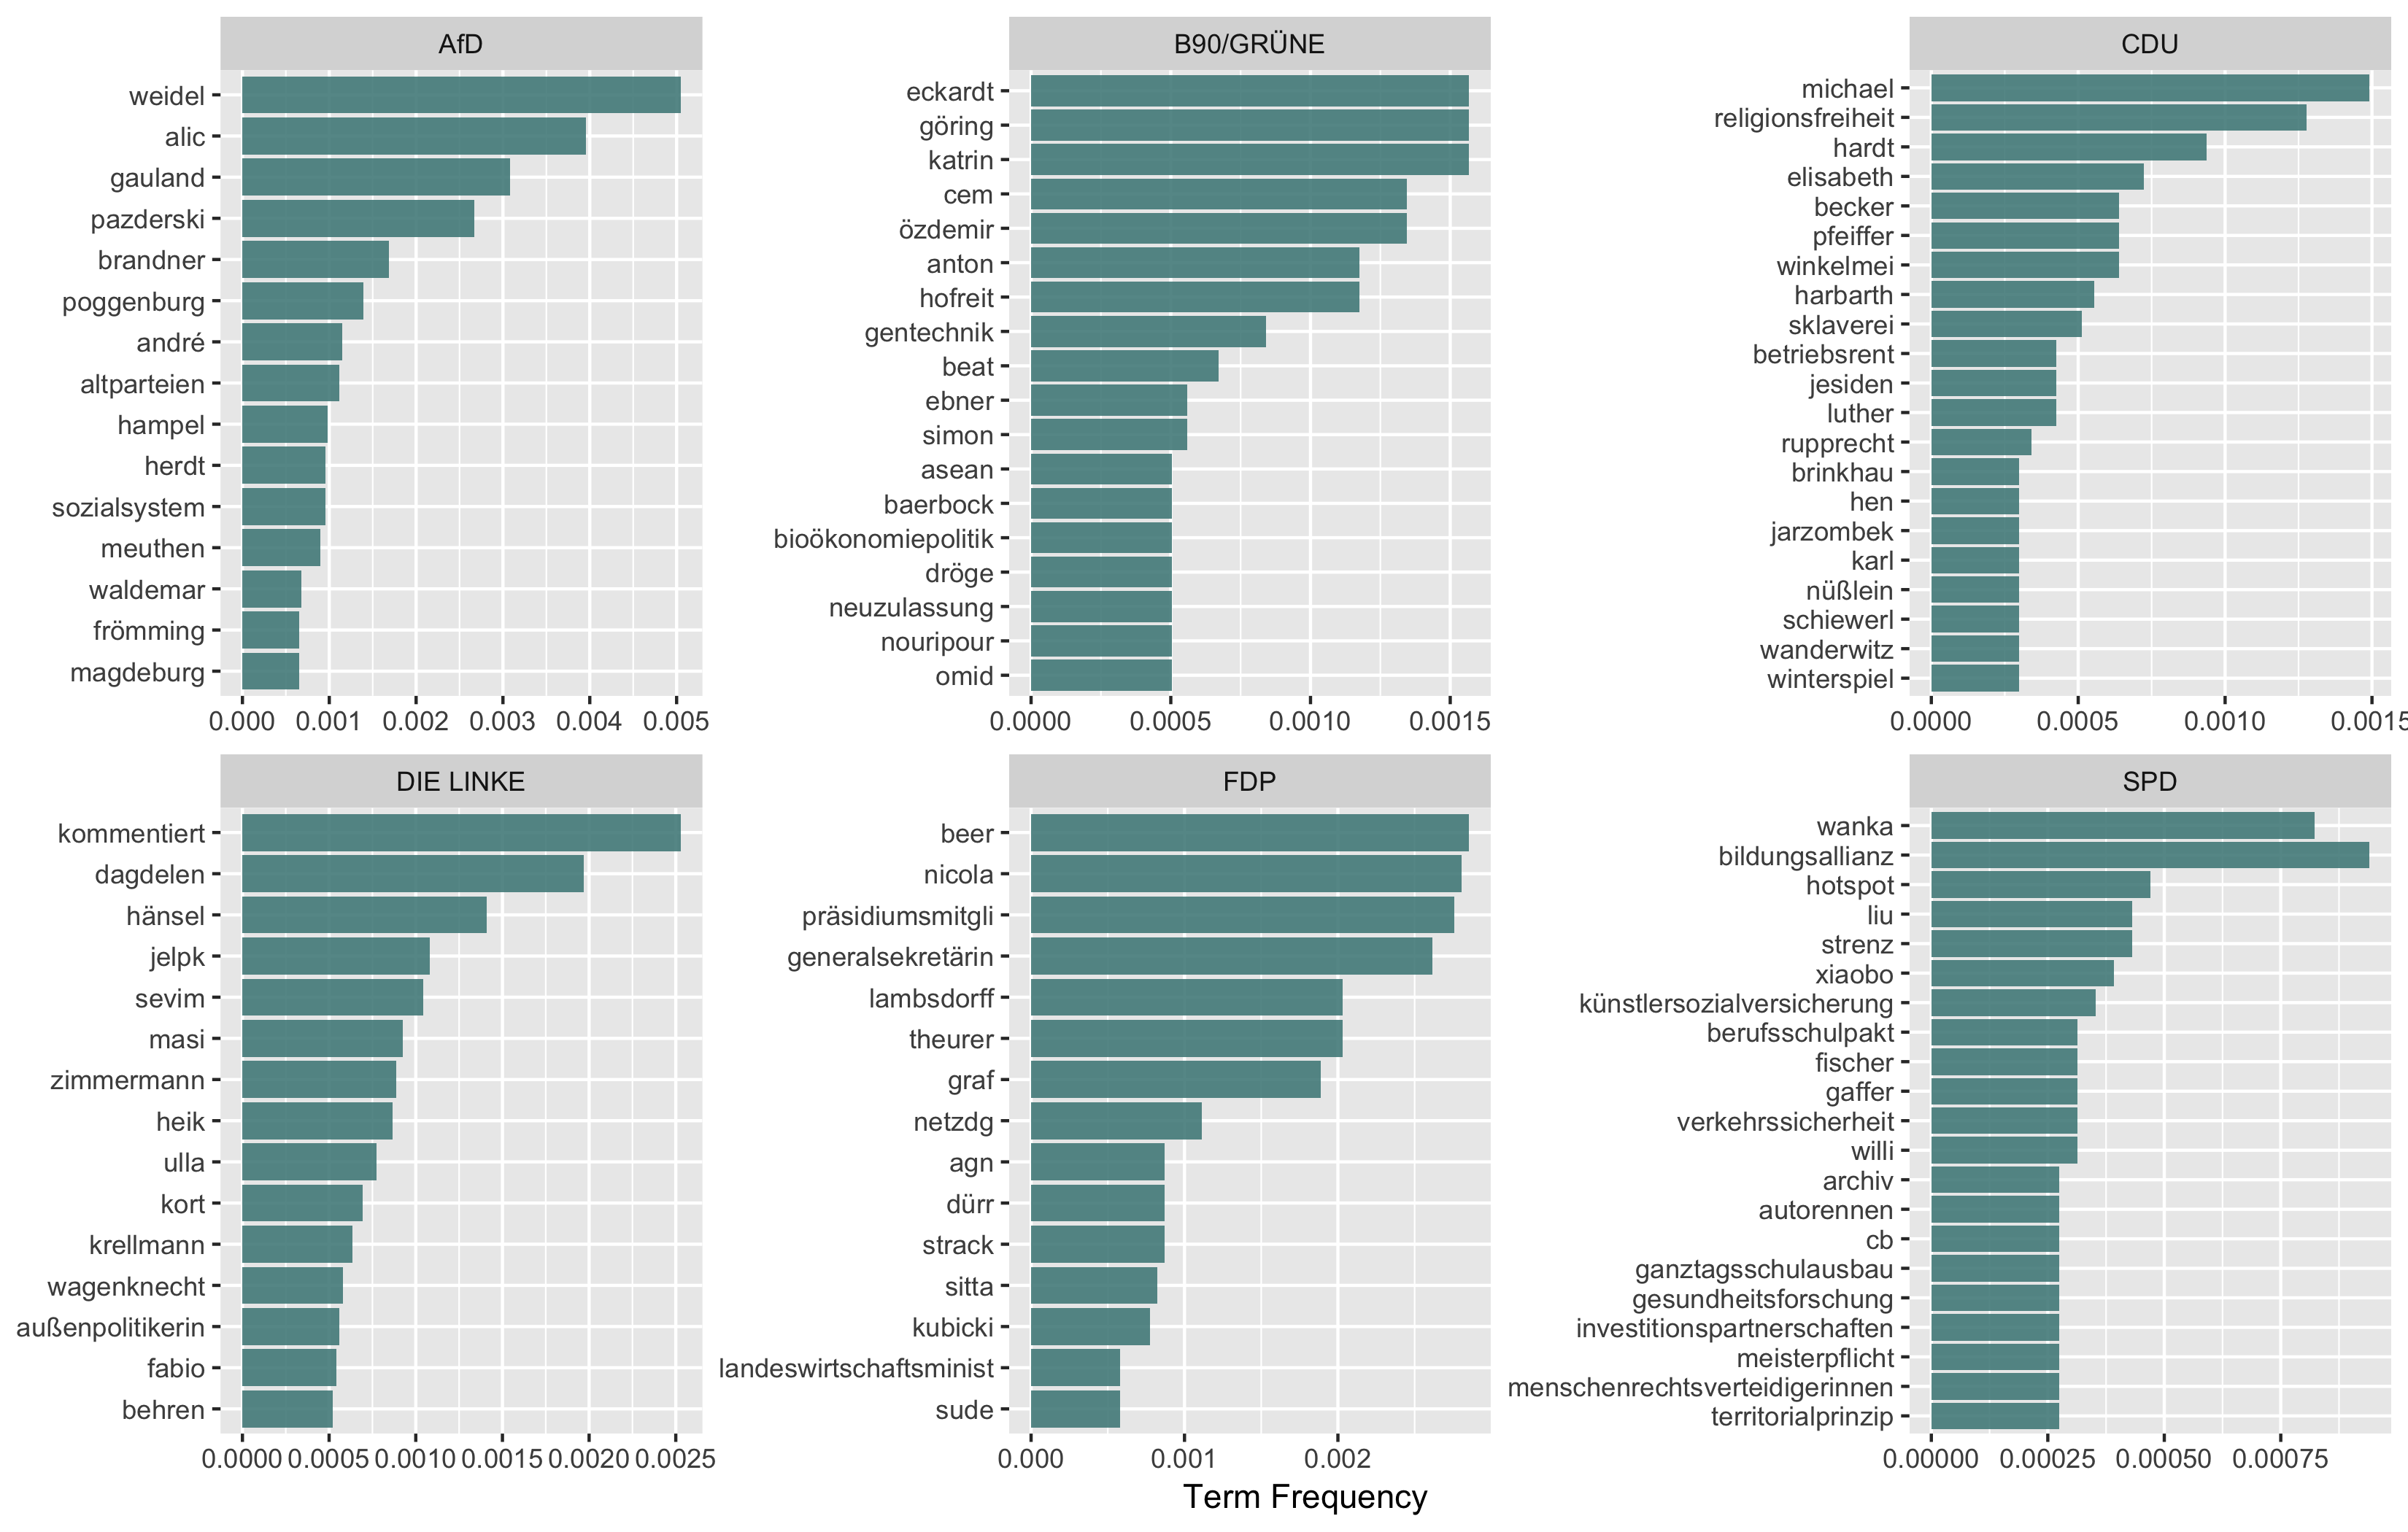
\includegraphics[width=\textwidth]{../figs/tokens}
	\label{fig_press}
	\end{center}
\end{figure}

\subsubsection{News articles}

% latex table generated in R 3.5.1 by xtable 1.8-3 package
% Sun Nov 11 21:36:13 2018
\begin{table}[ht]
\centering
\begin{tabular}{lrrr}
  \hline
medium & total\_articles & share & visits \\ 
  \hline
Bild.de & 3828 & 0.28 & 156867922 \\ 
  DIE WELT & 18663 & 0.14 & 52962285 \\ 
  FOCUS Online & 9235 & 0.22 & 68730873 \\ 
  SPIEGEL ONLINE & 5590 & 0.31 & 96139323 \\ 
  stern.de & 15804 & 0.15 & 18192672 \\ 
  tagesschau.de & 2261 & 0.41 & 75400000 \\ 
  ZEIT ONLINE & 5467 & 0.23 & 30600773 \\ 
   \hline
\end{tabular}
\caption{News sources used for the analysis} 
\end{table}


I conduct the estimation on a sample of 11,880 online news articles from seven German news providers about domestic politics\footnote{Bild.de, DIE WELT, FOCUS ONLINE, SPIEGEL ONLINE, stern.de, ZEIT ONLINE, Tagesschau.de}. The articles are dated from June 1, 2017 to March 1, 2018. I first extract all online articles using the Webhose.io API.\footnote{For more information see https://docs.webhose.io/v1.0/docs/getting-started. The scraping code was written in Python and can be made available on request.} Overall, the selected news providers are among the top ten German online news providers - in terms of site visits\footnote{The term visit is used to describe the call to a website by a visitor. The visit begins as soon as a user generates a page impression (PI) within an offer and each additional PI, which the user generates within the offer, belongs to this visit.} - in the period under review, with only Tagesschau.de belonging to the public media. The reason for this is that the content structure of Tagesschau.de is most similar to that of the private providers. Other public media offers provide their content in video (ZDF.de) or audio (Deutschlandfunk (DLF))) format, which make them difficult to compare. In order to limit the analysis to articles on domestic politics, all articles which mention at least one of the major parties\footnote{The exact search terms were "CDU, CSU, Union", "SPD", "FDP", "Grüne", "Linke", "AfD".} have been filtered out. 

 Figure \ref{fig_distr1} shows the distribution of the number of articles by date. There is a high peak around the federal elections on September, 24th and another one shortly after the failure of the Jamaica coalition talks on November, 19th (indicated by the red dotted lines). Figure \ref{fig_distr2} shows that DIE WELT published the most articles on domestic policy, followed by stern.de and FOCUS ONLINE.  

\begin{figure}[H]
	\caption{Article distribution...}
	\begin{center}
		\begin{subfigure}[normla]{0.59\textwidth}
			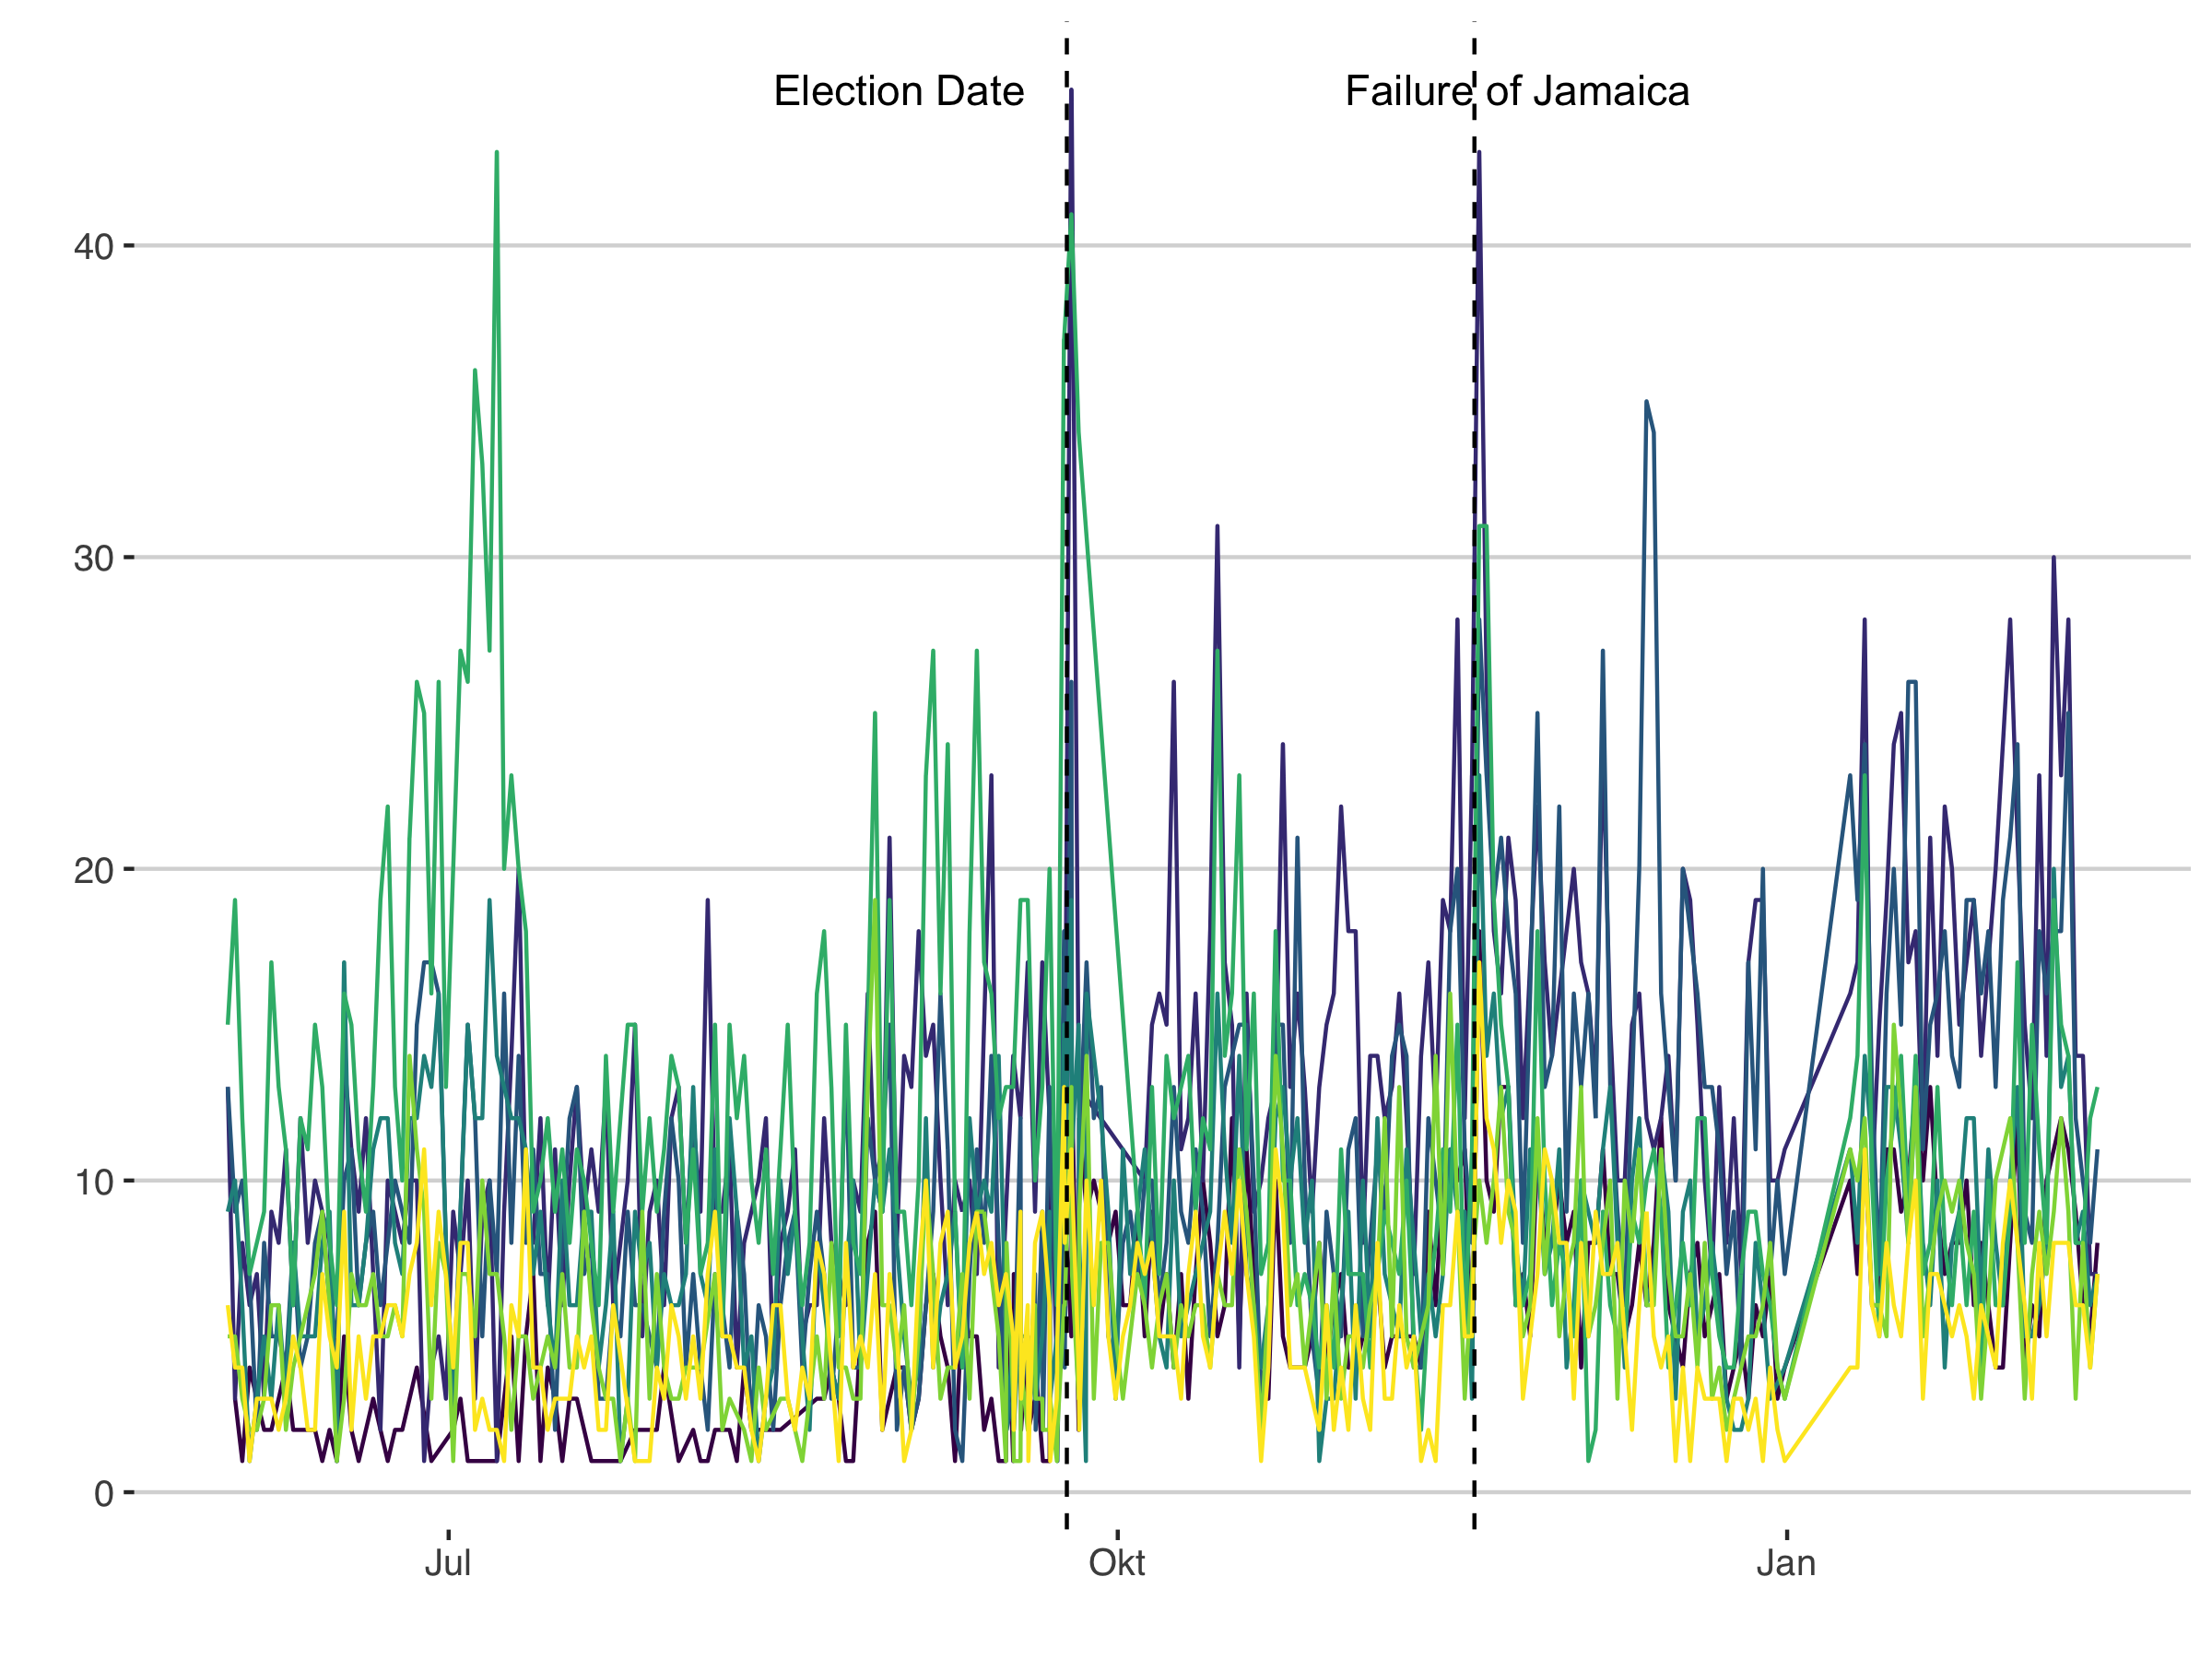
\includegraphics[width=\textwidth]{../figs/article_timeline.png}
			\caption{...by date}
			\label{fig_distr1}
		\end{subfigure}
		\begin{subfigure}[normla]{0.4\textwidth}
			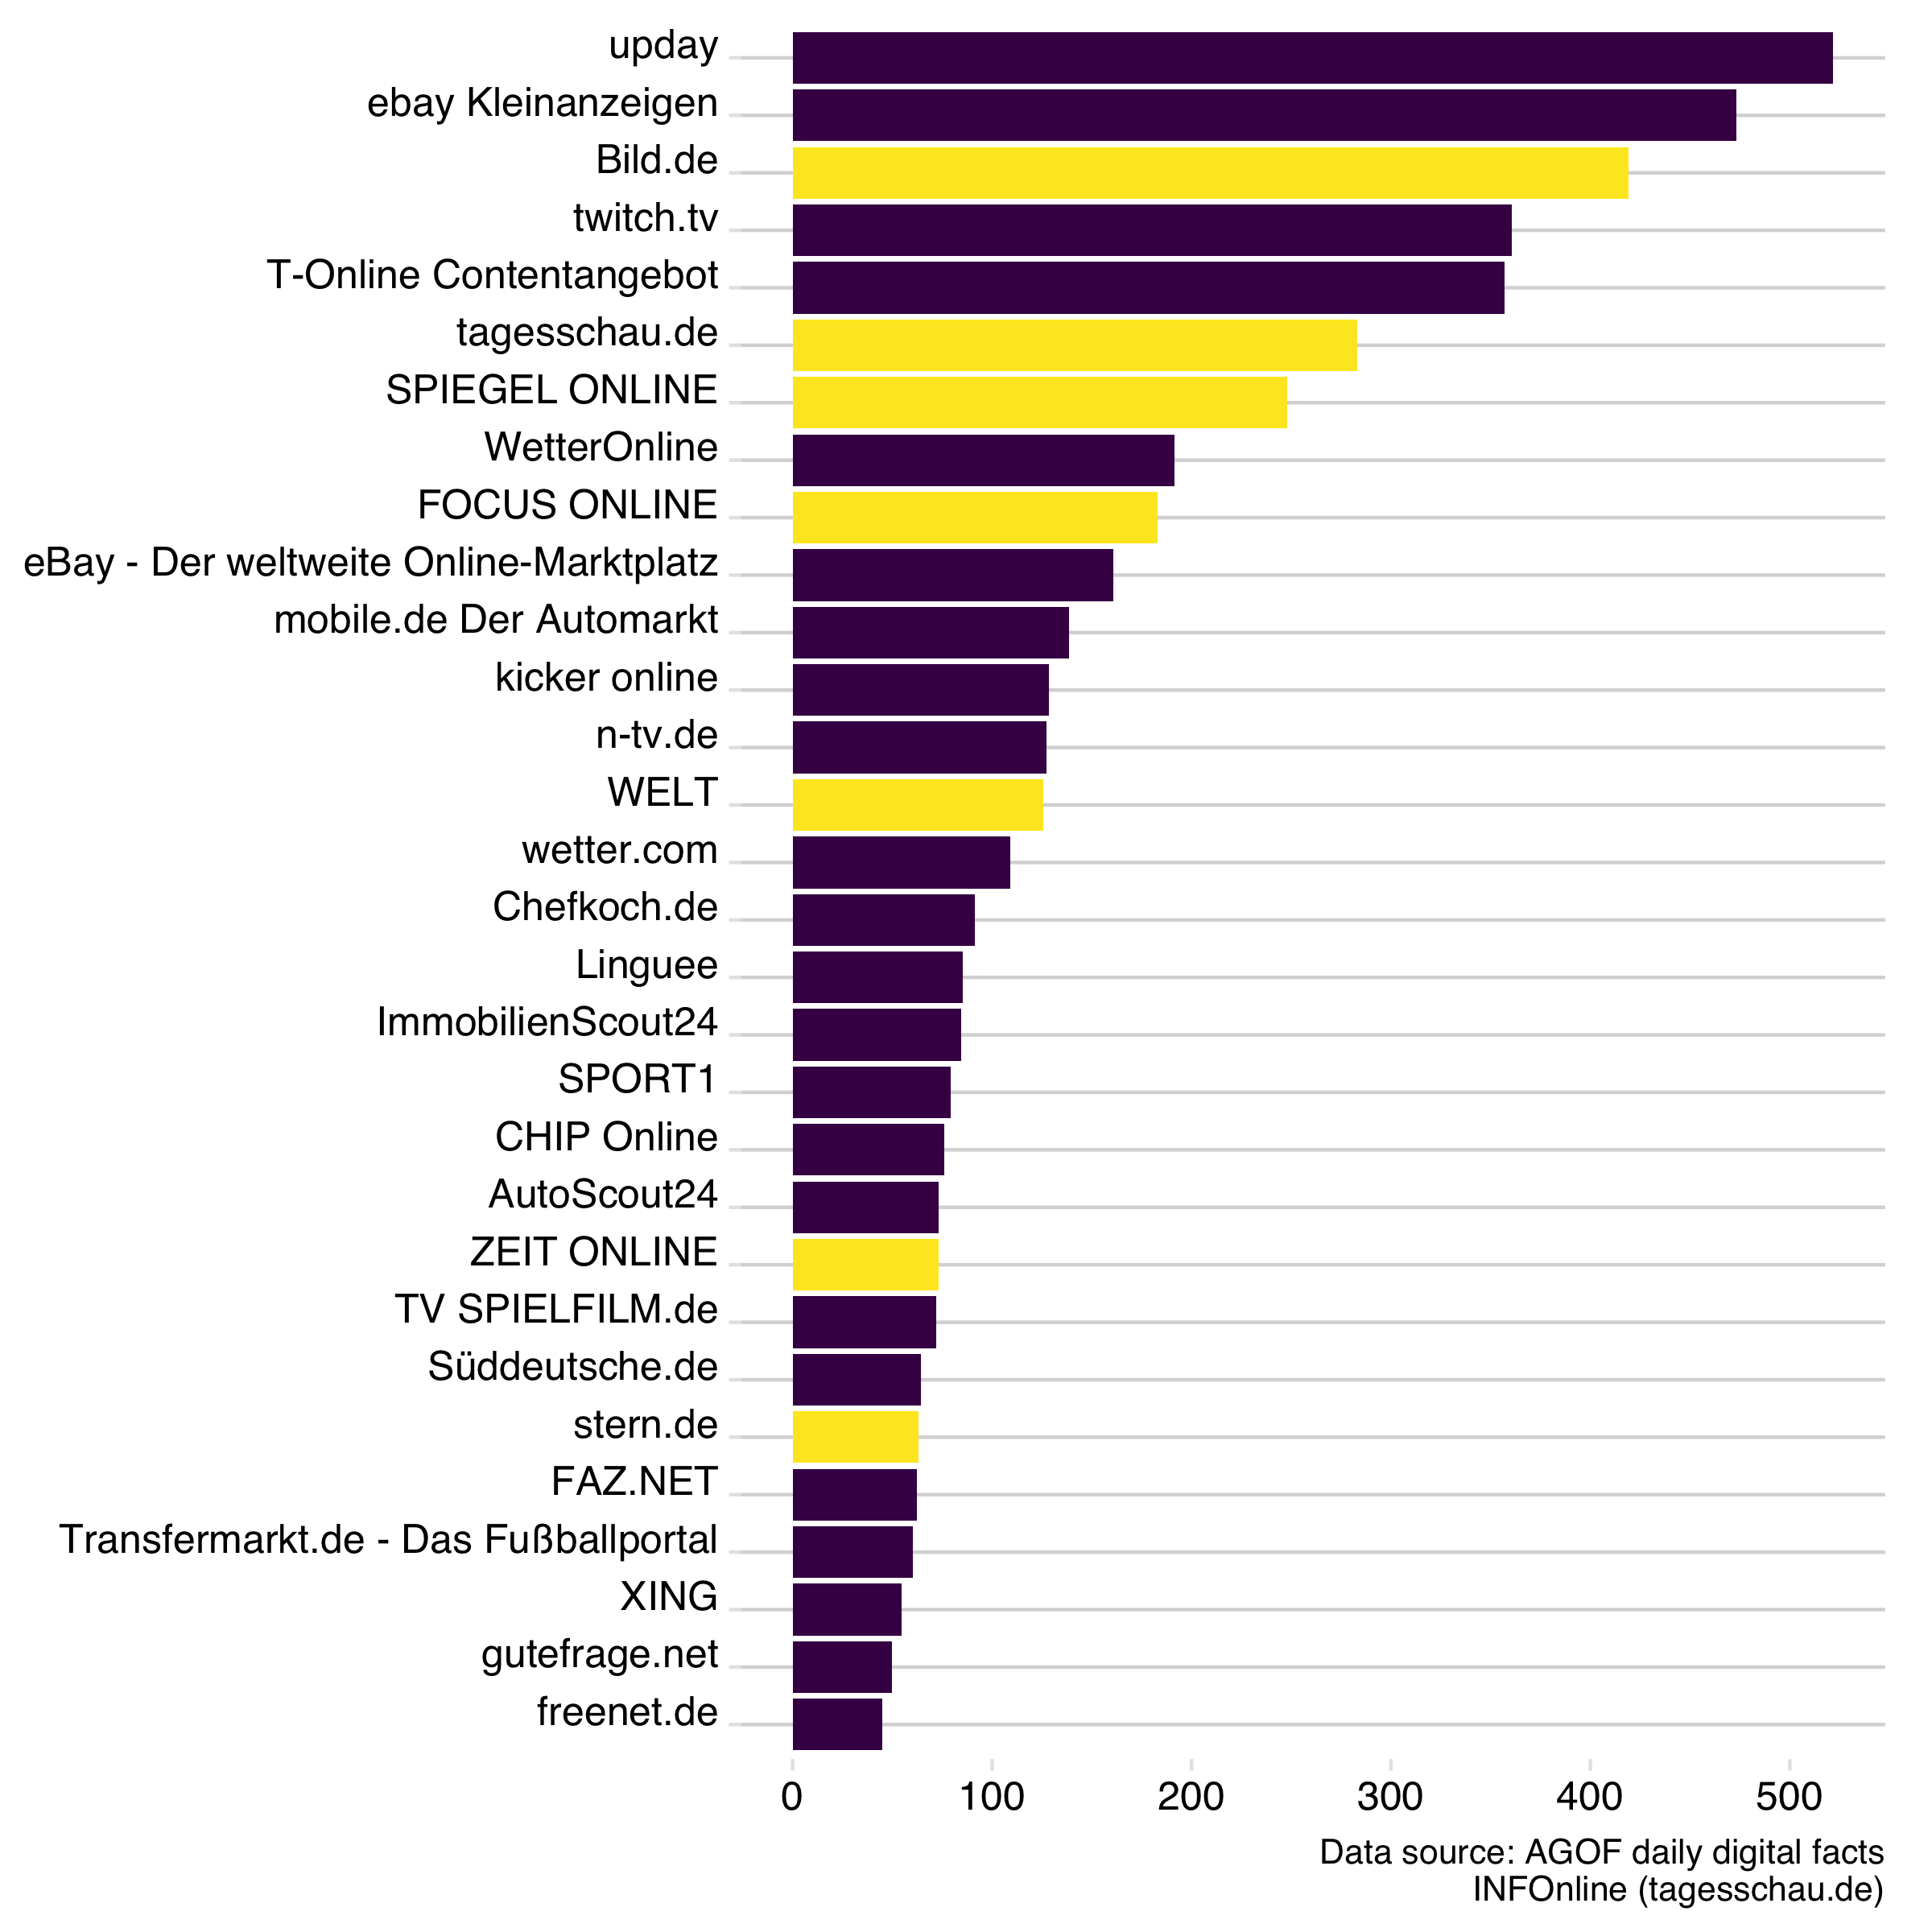
\includegraphics[width=\textwidth]{../figs/visits.png}
			\caption{... by news provider}
			\label{fig_distr2}
		\end{subfigure}
	\end{center}
\end{figure}

To allow for an operationalization of agenda bias, parties' press releases are used as an approximation of the potential universe of news stories \citep{eberl_one_2017}. The press releases were scraped from the website of each party\footnote{afd.de, spd.de, die-linke.de, fdp.de, gruene.de, cdu.de} and each faction\footnote{afdbundestag.de, spdfraktion.de, die-linke.de/start/presse/aus-dem-bundestag, fdpbt.de, gruene-bundestag.de/, presseportal.de/nr/7846} to compare the topics addressed with the policy issues in the news articles. 



\subsubsection{Data preparation}

To use text as data for statistical analysis, different pre-processing steps have to be conducted. In fact, in order to use text as data and reduce the dimensionality to avoid unnecessary computational complexity and overfitting, pre-processsing the text is a central task in text mining \citep{bholat_text_2015}. Intuitively the term frequency (tf) of a word is a measure of how important that word may be for the understanding of the text. As can be seen in Figure \ref{fig_wordcloud1}, problems arise with words that are highly frequent. For example "die", or "der (eng. "the"), "und" (eng. "and"), and "ist" (eng. "is") are extremely common but unrelated to the quantity of interest. These terms, often called stop words \citep{gentzkow_text_2017}, are important to the grammatical structure of a text, but typically don't add any additional meaning and can therefore be neglected. A common strategy to reduce the number of language elements is to pre-process the text by imposing some preliminary restrictions (e.g. stop-word removal and stemming) based on the nature of the data (e.g. twitter text, newspaper articles, speeches, etc.) \citep{gentzkow_text_2017}. 

To remove distorting words, the pre-defined stop word list from the Snowball project\footnote{http://snowball.tartarus.org/algorithms/german/stop.txt} is used together with a customized list of stop-words. Additionally punctuation character (e.g. ., ,, !, ?, etc.) and all numbers are removed from the data. A next step to reduce the dimensionality of text data is to apply an adequate stemming technique. Stemming is a process by which different morphological variants of a word are traced back to their common root. For example, "voting" and "vote" would be treated as two instances of the same token after the stemming process. There are many different techniques for the stemming process. I apply the widely used Porter-Stemmer algorithm, which is based on a set of shortening rules that are applied to a word until it has a minimum number of syllables.\footnote{https://tartarus.org/martin/PorterStemmer/} After completing these steps 68,576 unique terms were left in the vocabulary. The word clouds in Figure \ref{fig_wordcloud2} represent the most frequent words of the pre-processed articles for Bild.de and Tagesschau.de. It becomes evident that these are texts discussing domestic policy issues. The SPD in particular seems to be highly frequent. However, at first glance, there are no obvious differences between the news providers.  

 % --------------------
% Document-term-matrix
% --------------------
The next step is to divide the entire dataset into individual documents and to represent these documents as a finite list of unique terms. In this setting, each news article and each press release represents a document $d$, whereby each of these documents can be assigned to a news website or a party. The sum of all documents forms what is called the corpus. For each document $d \in \lbrace 1,...,D \rbrace$ the number of occurrences of term $v$ in document $d$ is computed, in order to obtain the count $x_{d,v}$, where each unique term in the corpus is indexed by some $v \in \lbrace 1,...,V \rbrace$ and where $V$ is the number of unique terms. The $D$ x $V$ matrix $\boldsymbol{X}$ of all such counts is called the document-term matrix. Each row in this matrix represents a document, where each entry in this row counts the occurrences of a unique term in that document. This representation is often referred to as the bag of words model \citep{gentzkow_text_2017}, since the order in which words are used within a document is disregarded.

\subsubsection{Structural topic model}

To find out the latent structure of each document, a structural topic model (STM) is estimated. In general, topic models formalize the idea that documents are formed by hidden variables (topics) that generate correlations among observed terms. They belong to the group of unsupervised generative models, meaning that the true attributes (topics) cannot be observed. One crucial assumption to be made for such models is the number of topics ($K$) that occur over the entire corpus. 

Each individual topic potentially contains all of the unique terms within the vocabulary $V$ with different probability. Therefore, each topic $k$ can be represented as a probability vector $\phi_k$ over all unique terms $V$. Simultaneously, each individual document $d$ in the corpus can be represented as a probability distribution $\theta_d$ over the $K$ topics. The underlying data generating process to generate each individual word $w_{d,n}$ in a document $d$ for the $n^{th}$ word-position can be described as follows:\footnote{A more detailed description of the generative process of the STM can be found in section \ref{ch_generativeProcess}}

\begin{enumerate}
	\item for each document $i$, draw its distribution of topics $\theta_d$ depending on the metadata included in the model; 
	\item for each topic $k$, draw its distribution of words $\phi_k$ depending on the metadata included in the model;
	\item for each word $n$, draw its topic $z_n$ based on $\theta_i$;
	\item for each word word $n$, draw the term distribution for the selected topic $\phi_{z_{d,n}}$.
\end{enumerate}

% ----------------------
% Model Selection
% ----------------------
Inference of mixed-membership models, such as the one applied in this paper, has been a thread of research in applied statistics in the past few years (\citet{blei_latent_2003} \citet{erosheva_mixed-membership_2004} \citet{braun_variational_2010}). Topic models are usually imprecise as the function to be optimized has multiple modes, such that the model results can be sensitive to the starting values (e.g. the number of topics). Since an ex ante valuation of a model is hardly possible, I compute a variety of different models and compare their posterior probability. This enables me to check how results vary for different model solution \citep{roberts_navigating_2016}. I then cross-checked some subset of assigned topic distributions to evaluate whether the estimates align with the concept of interest \citep{gentzkow_text_2017}. These manual audits are applied together with numeric optimization based on the topic coherence measure suggested by \citet{mimno_optimizing_2011}. 

This process revealed that a model with 60 topics best reflects the structure in the corpus. Furthermore, the source (news website or party) of a document is used as covariate in the topic prevalence. In other words, the corresponding news website or party of an article or press release influences the probability distribution of topics for that document. Additionally I assume that the topical content differs between news articles and press releases. 

% ---------------------- 
% ------- Results 
% ---------------------- %

\section{Results}

\subsection{Topic distribution} 

The generative process of the STM results in two posterior distributions: (1) a distribution over all topics for each document and (2) a distribution over all words for each topic. As we included the type of source (news article or press release) as a covariate in the model, we have two different posterior word-distributions for each topic. A combination of both is used to label the topics as listed in table \ref{t_labels}. 
 
For each document, we have a distribution over all topics

\begin{figure}[H]
\begin{center}
	\caption{Document-Topic distribution}
	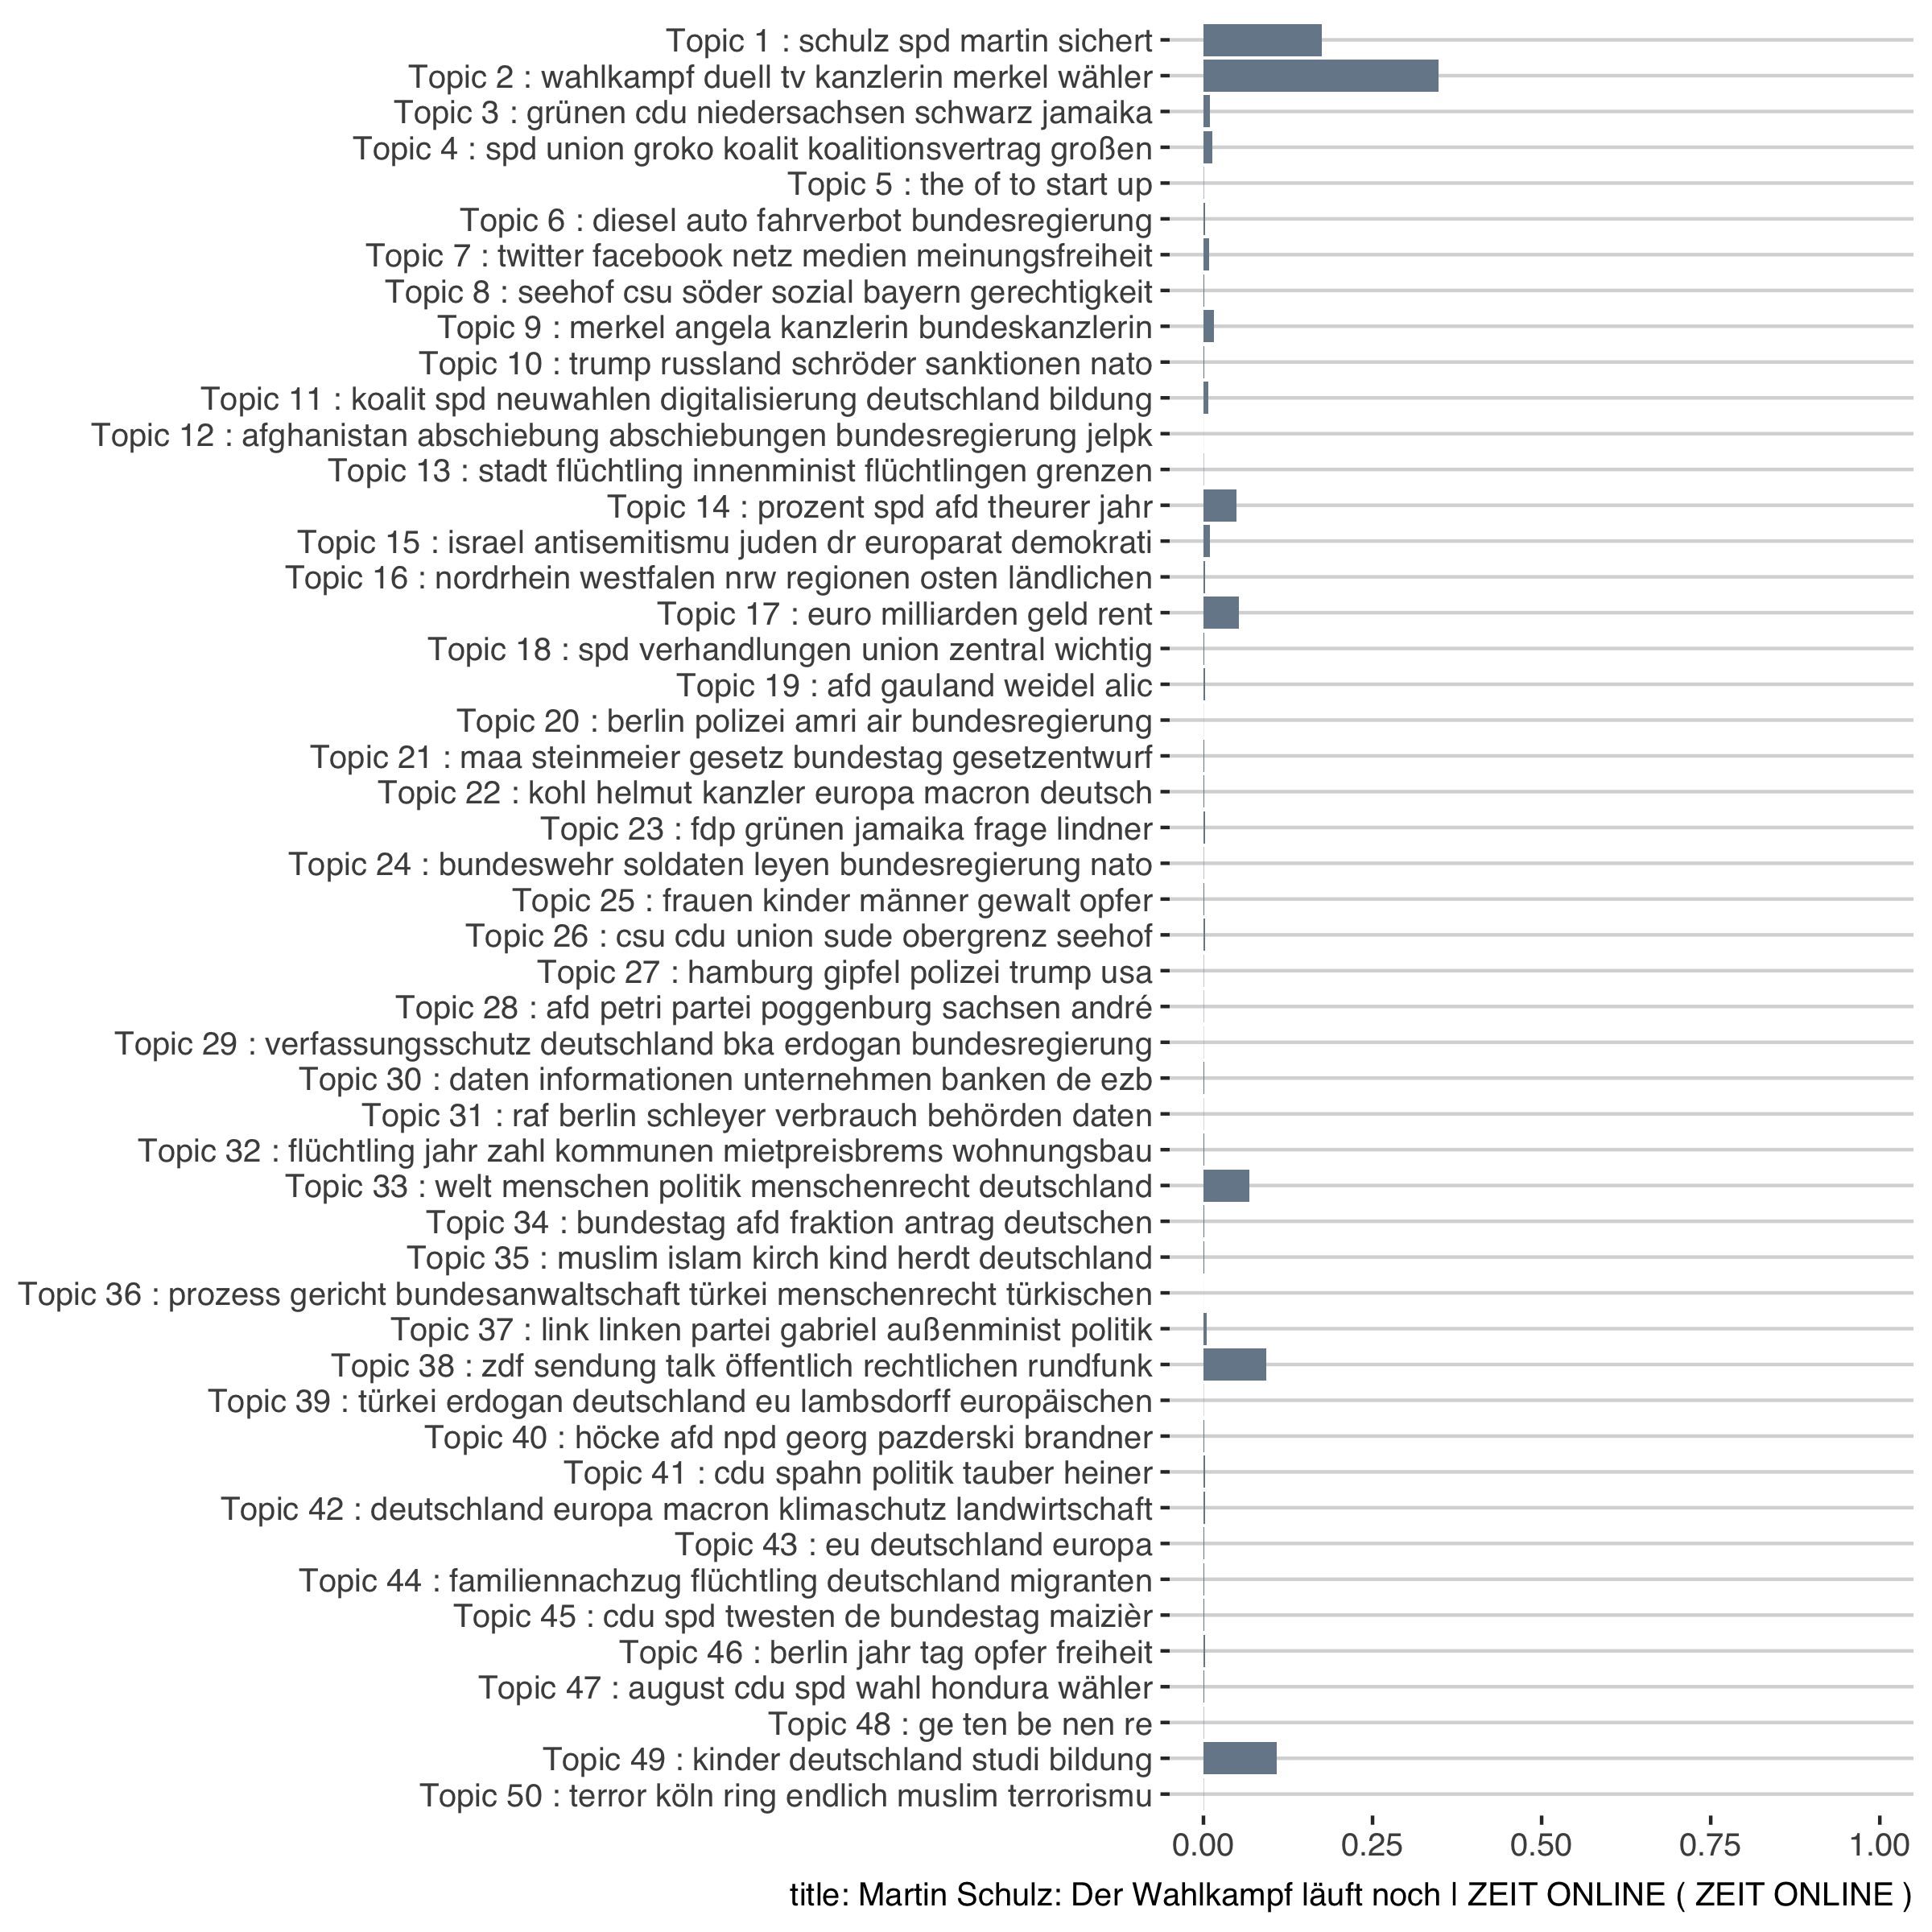
\includegraphics[width=\textwidth]{../figs/doc_topic_distr}
	\label{fig_doc_topic_distr}
	\end{center}
\end{figure}

The average of all documents gives the expected frequency of a topic in the whole corpus as shown in figure \ref{fig_expected_freq}

\begin{figure}[H]
\begin{center}
	\caption{Document-Topic distribution}
	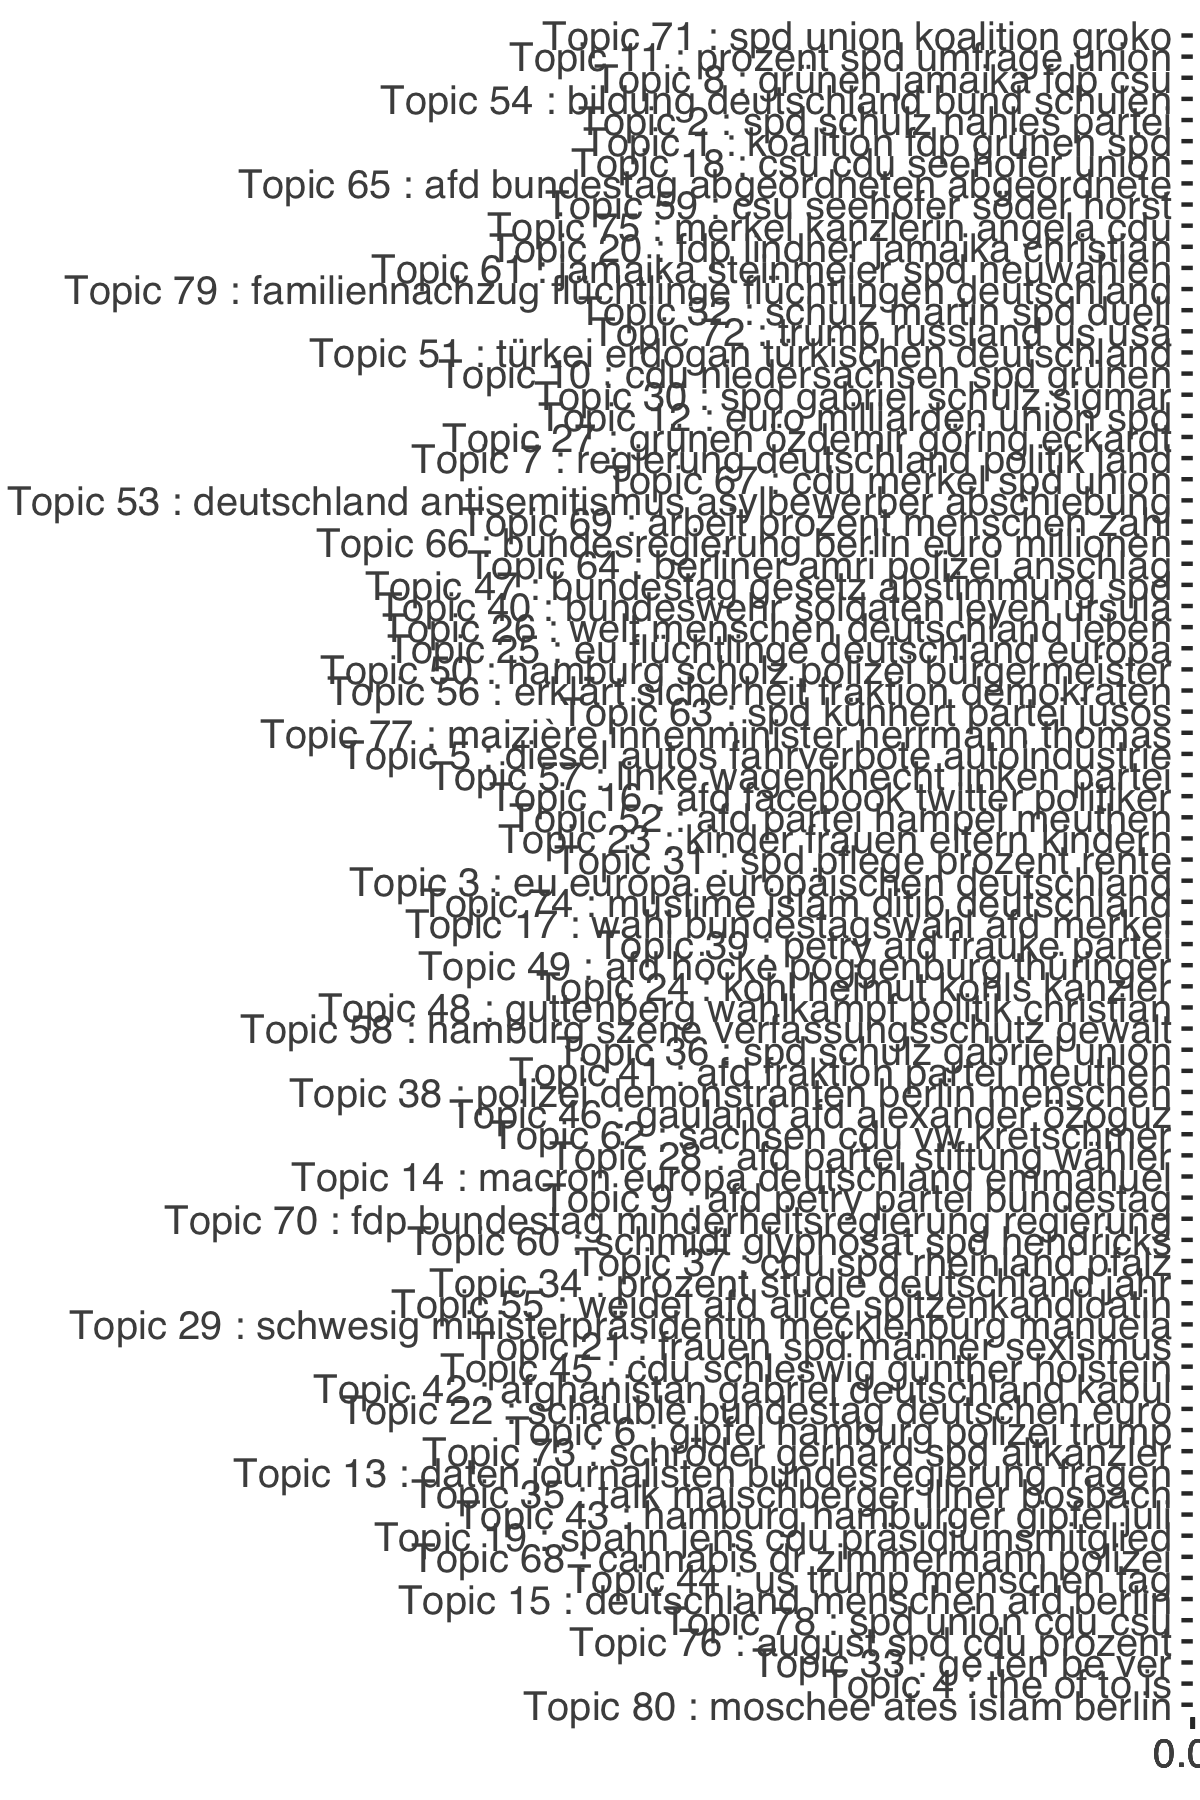
\includegraphics[width=\textwidth]{../figs/topic_proportion}
	\label{fig_expected_freq}
	\end{center}
\end{figure}

It becomes apparent that topic 20 about the so-called Jamaica parties (CDU/CSU, FDP and B90/Die Grünen) is the topic with the highest expected frequency in the whole corpus, followed by topic 36 about the coalition talks between CDU/CSU and SPD - the "Grand coalition" or "GroKo". However, the model was calculated under the assumption that each document source has a different distribution across all topics. Looking at the expected frequency of a topic for each source separately, some differences become apparent.

\begin{figure}[H]
	\caption{Expected frequency}
	\begin{center}
		\begin{subfigure}[normla]{0.48\textwidth}
			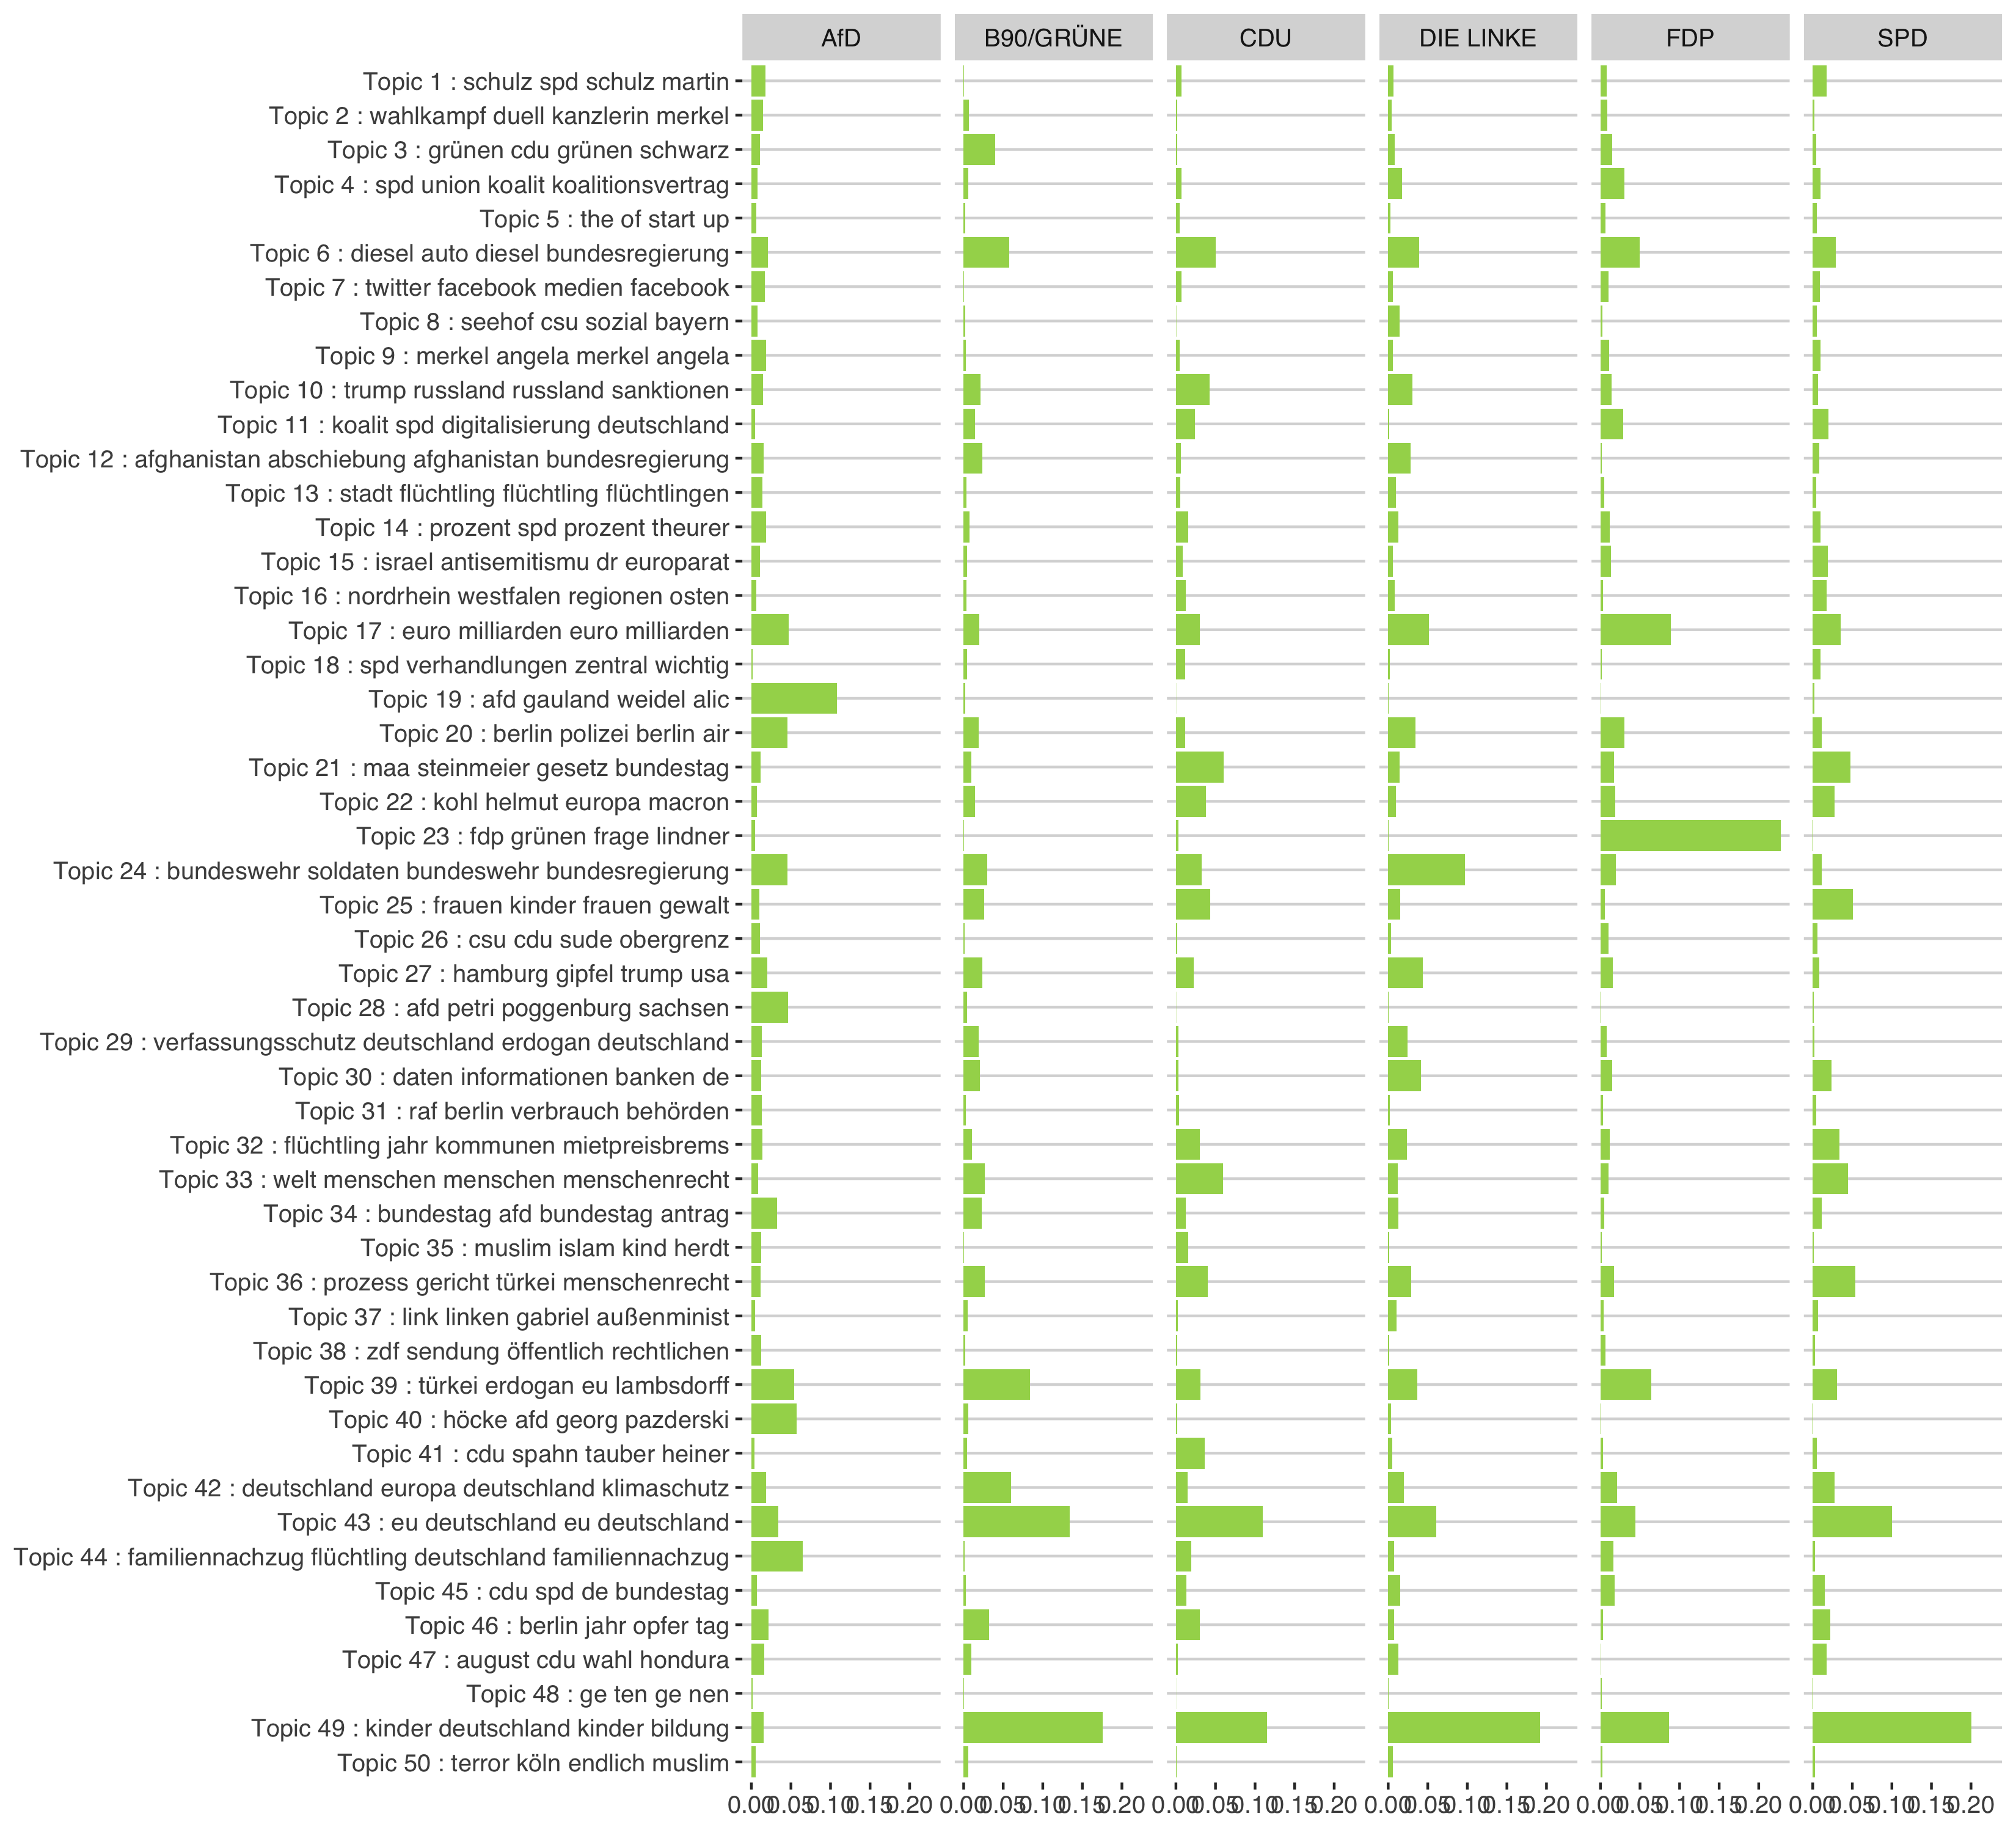
\includegraphics[width=\textwidth]{../figs/topic_proportion_press}
			\caption{Online news}
		\end{subfigure}
		\begin{subfigure}[normla]{0.48\textwidth}
			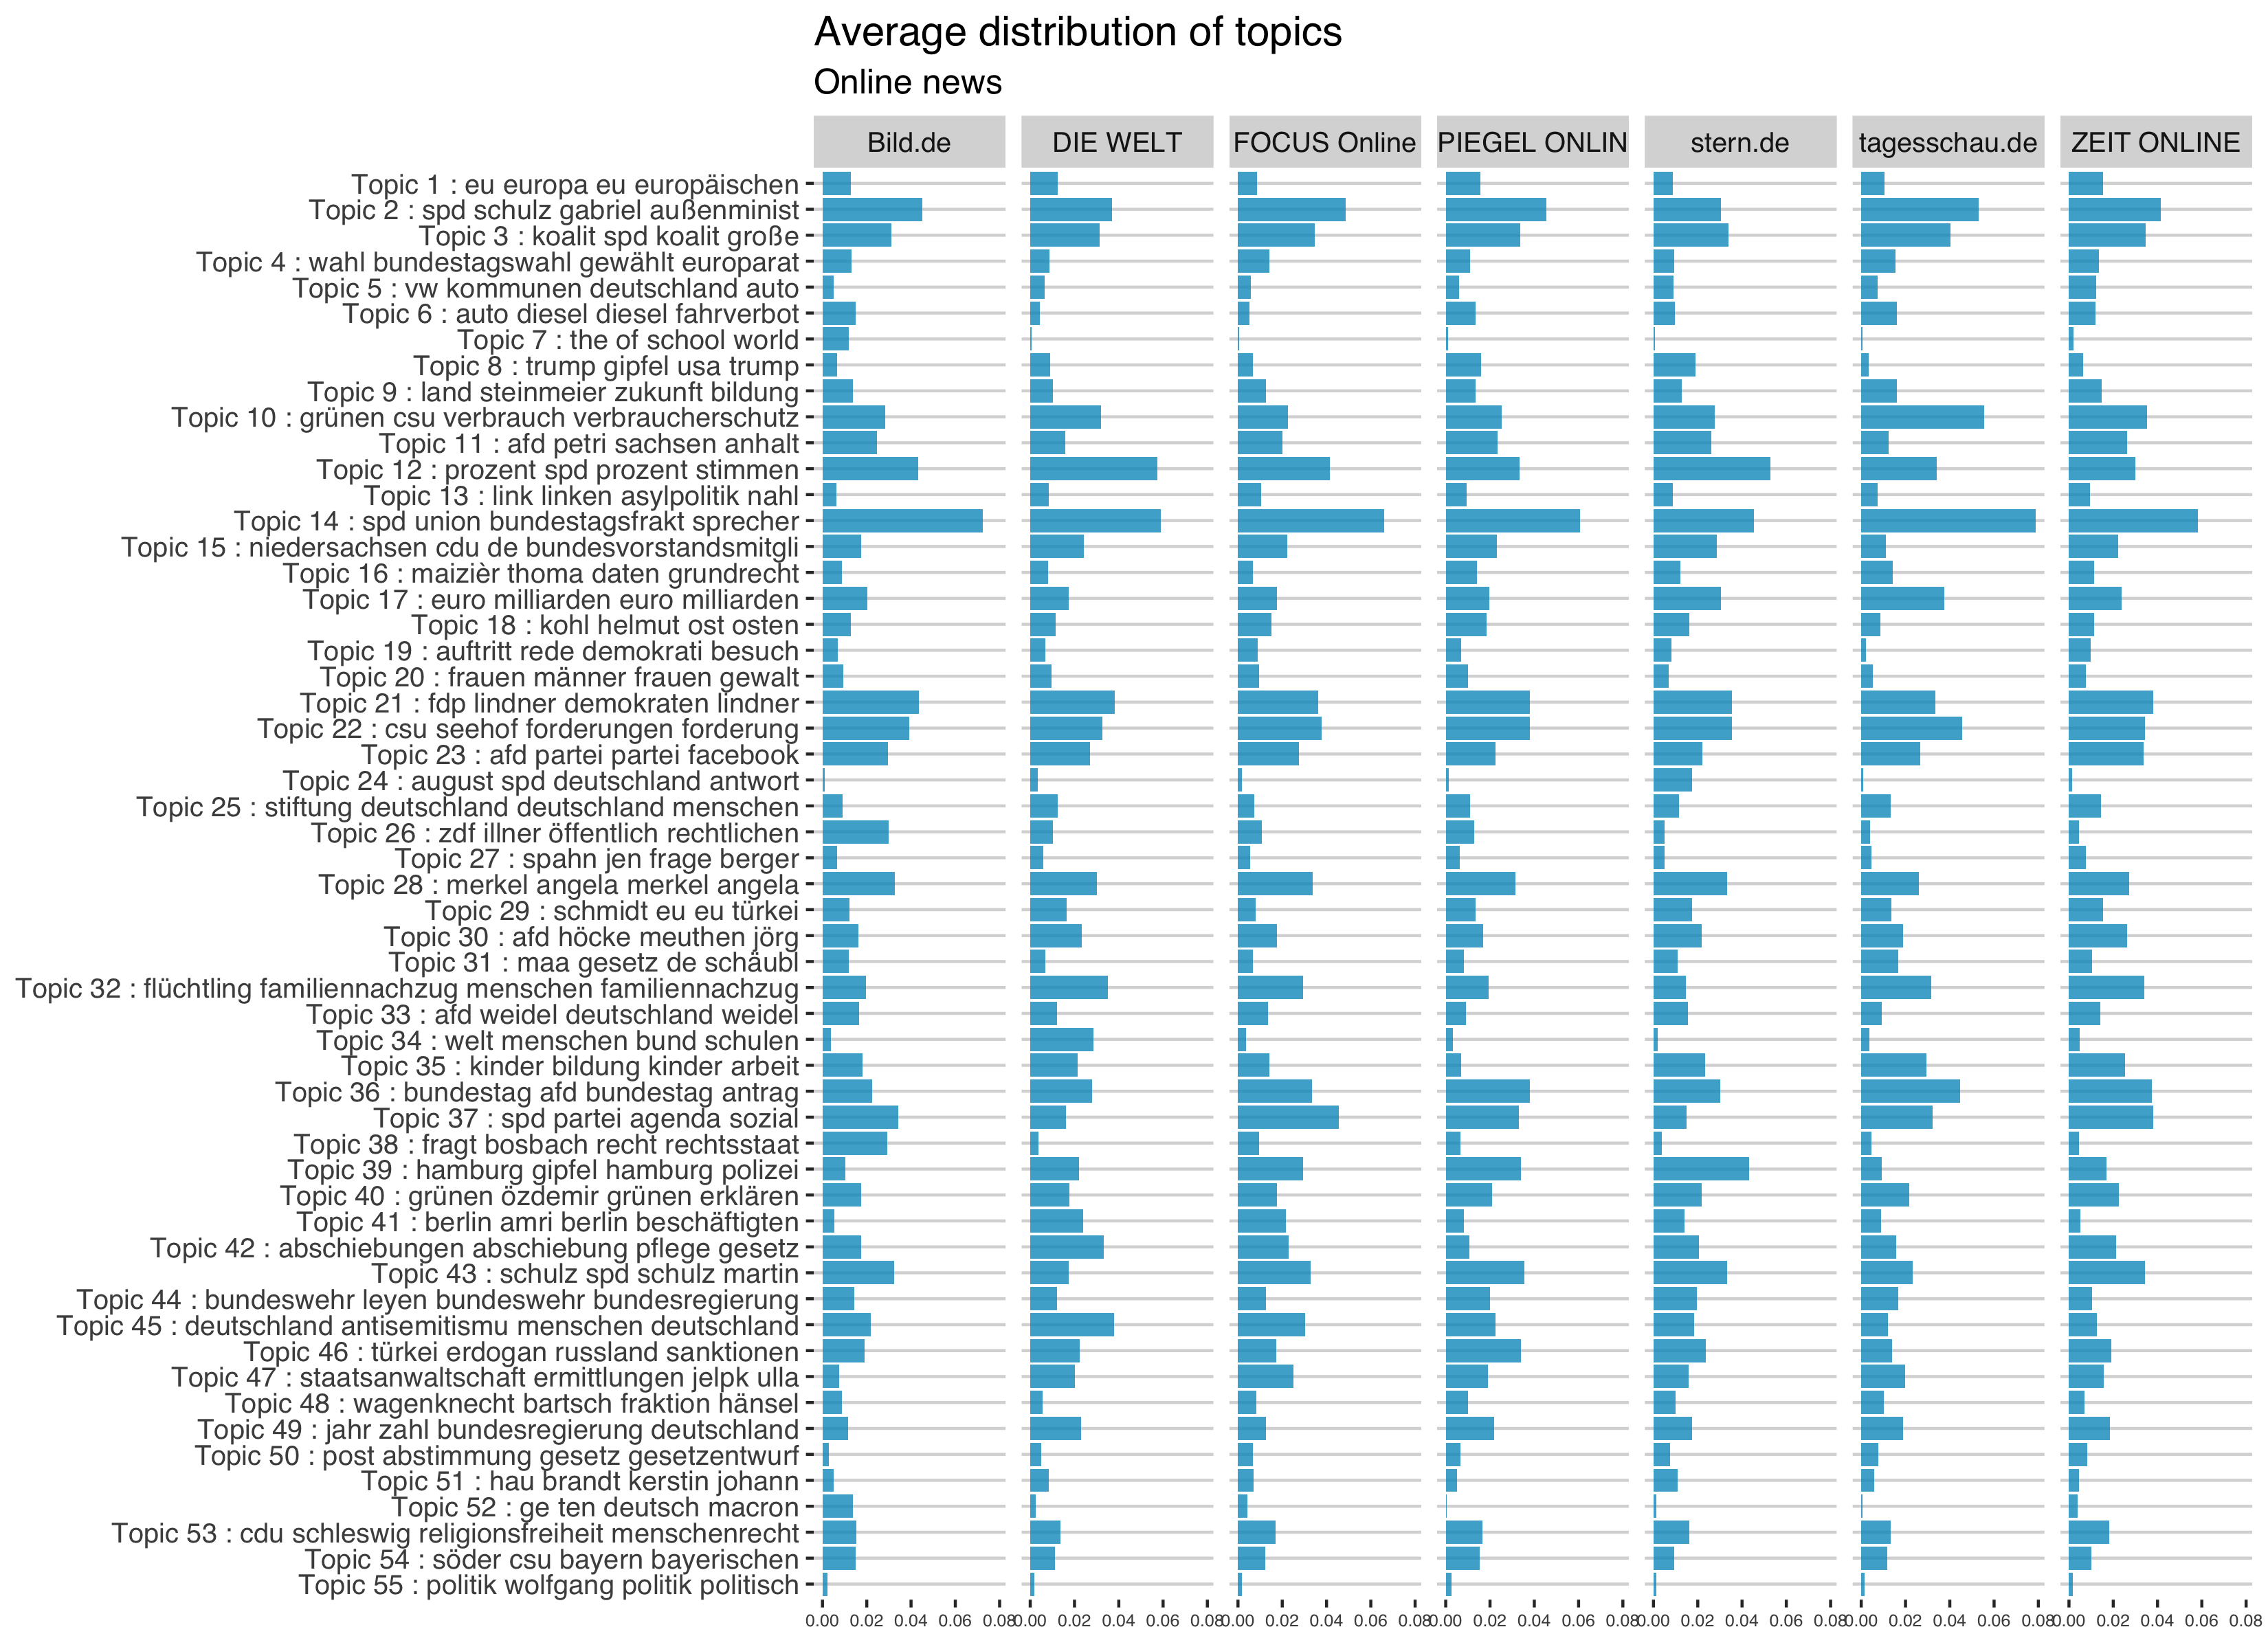
\includegraphics[width=\textwidth]{../figs/topic_proportion_news}
			\caption{Press releases}
		\end{subfigure}
	\end{center}
\end{figure}

\subsection{Agenda correlation}

Agendas were measured in terms of percentage distributions across the 80 topics. For each source the average distribution of each topic is calculated for each month. The following pictures show the overall topic distribution. Then, we estimated bivariate correlations between party agendas and the mediated party agendas in the online news. These correlations represent the agenda selectivity each party experiences in each media outlet. The higher the correlation, the more congruent both agendas are. 

\begin{figure}[H]
\begin{center}
	\caption{Document-Topic distribution}
	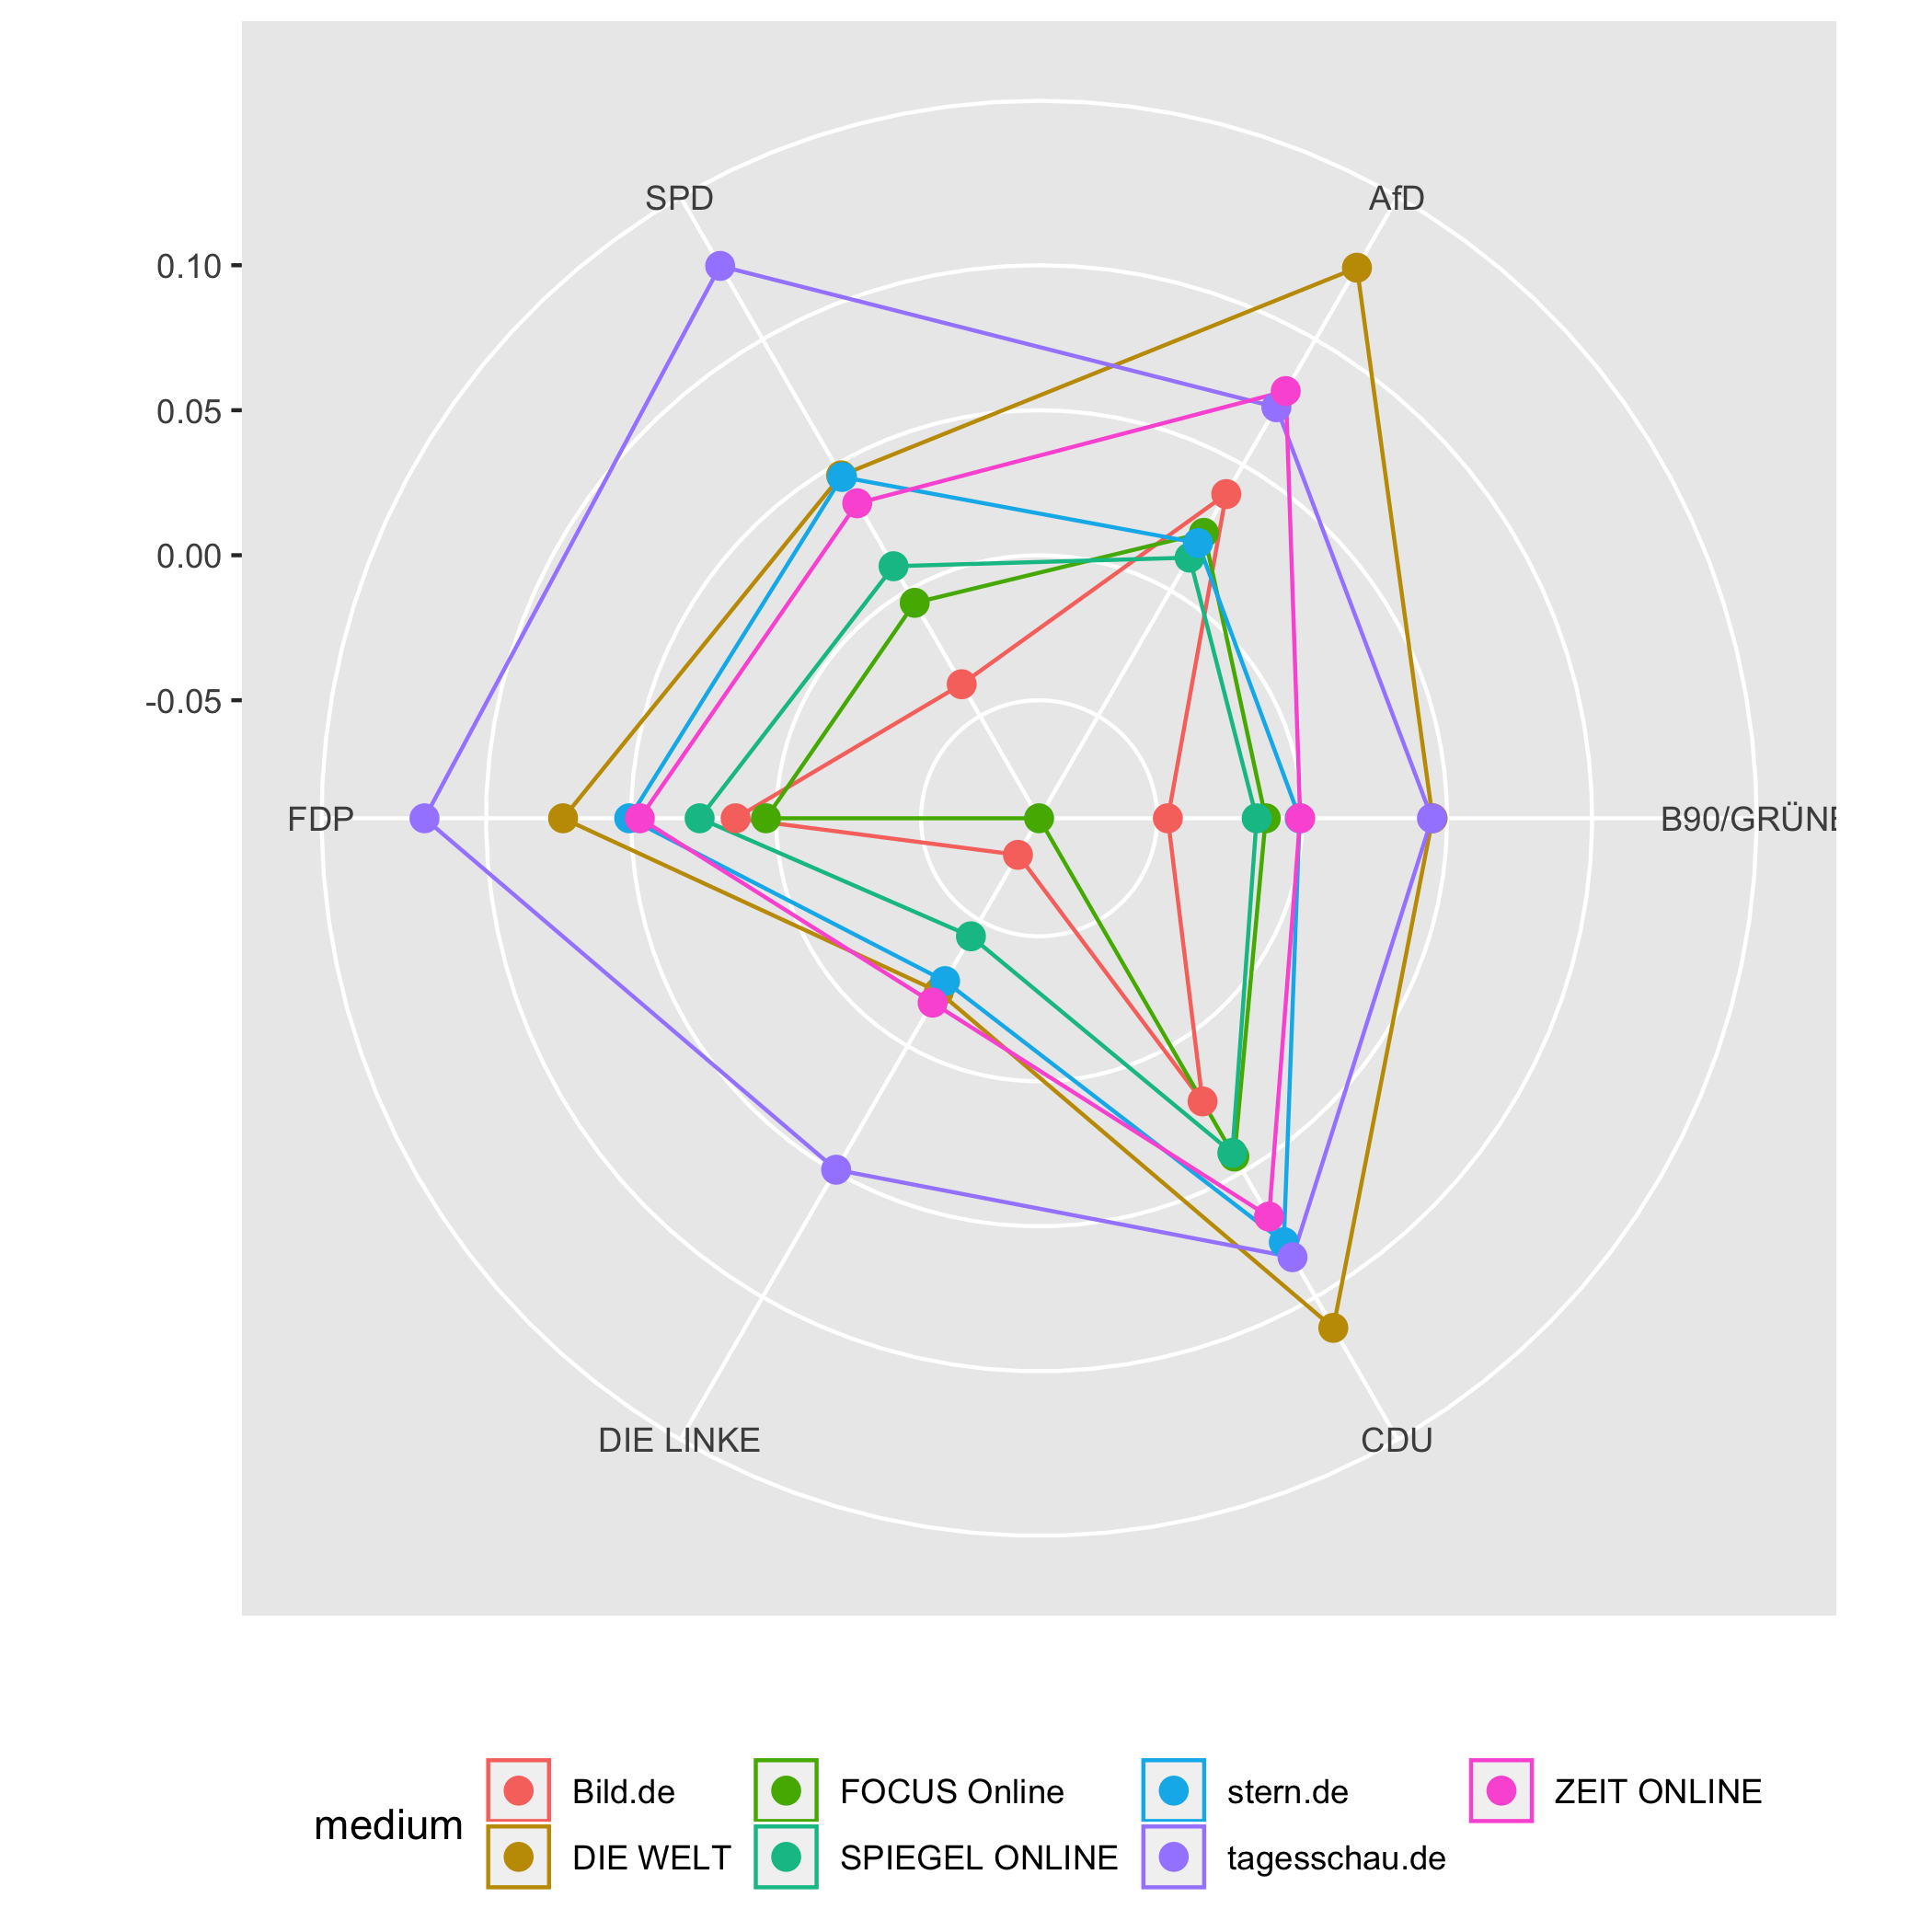
\includegraphics[width=\textwidth]{../figs/radarchart}
	\label{fig_expected_freq}
	\end{center}
\end{figure}

\section{Conclusion}

The ongoing discussion about the influence of digital media on the political opinion-forming process addresses the question whether there are convergence tendencies within the mass media and whether the reporting in the media correlates with the voting preferences. To analyze this question, this paper examines .... 

Using text data of 14,937 online news articles from seven German news providers about domestic politics, I first estimate a Structural Topic Model to find the latent topics in the news articles ...

\pagebreak

\printbibliography

\appendix
\section{Appendices}

\subsection{Generative Process of STM}\label{ch_generativeProcess}

 The following describes the generative process for filling the $n^{th}$ word-position in document $d$ in the case of the STM \citep{roberts_structural_2013}: As in the case of conventional models, first a specific topic $z_{dn}$ is assigned, according to the topic distribution for that document $\theta$ through the process:

\begin{equation}
	z_{dn}|\theta_d \sim \textrm{Multinomial}(\theta_d).
\end{equation}

To incorporate the covariate values for that document, a topic-prevalence vector $\theta_d$ is drawn from a logistic-normal distribution:

\begin{equation}
	\theta_d|y_{d\gamma},\Sigma \sim \textrm{LogisticNormal}(\mu = y_{d\gamma}\Sigma),
\end{equation}

where $y_d\gamma$ lists the values of the metadata covariates for document $d$ and $\gamma$ relates these covariate values to the topic-prevalence. 

Conditional in the topic chosen ($z_{dn}$), a specific word $w_{dn}$, is selected from the overall corpus vocabulary $V$, using the following process:

\begin{equation}
	w_{dn}|z_{dn},\phi_{dkv} \sim \textrm{Multinomial}(\phi_{dk1},...,\phi_{dkV}),
\end{equation}

where the word probability $\phi_{dkv}$ is parameterized in terms of log-transformed rate deviations from the rates of a corpus-wide background distribution $m_v$ \citep{roberts_structural_2013}. The log-transformed rate deviations can then be specified by a collection of parameters $\lbrace \boldsymbol{\kappa} \rbrace$, where $\kappa^{(t)}$ is a $K$-by-$V$ matrix containing the log-transformed rate deviations for each topic $k$ and term $v$, over the baseline log-transformed rate for term $v$. This matrix is the same for all $A$ levels of covariates. To put it differently, $\kappa^{(t)}$ indicates the importance of the term $v$ given topic $k$ regardless of the covariates. Similarly, $\kappa^{(c)}$ is a $A$-by-$V$ matrix, indicating the importance of the term $v$ given the covariate level $c$ regardless of the topic. Finally, $\kappa^{(i)}$ is a $A$-by-$K$-by-$V$ matrix, collecting the covariate-topic effects:

\begin{equation}
	\phi_{dkv}|z_{dn}=\frac{\textrm{exp}(m_v+\kappa^{(t)}_{kv},\kappa^{(c)}_{y_dv}+\kappa^{(i)}_{y_dkv})}{\sum_v \textrm{exp}(m_v+\kappa^{(t)}_{kv},\kappa^{(c)}_{y_dv}+\kappa^{(i)}_{y_dkv})}.
\end{equation}

The STM maximizes the posterior likelihood that the observed data were generated by the above data-generating process using an iterative approximation-based variational expectation-maximization algorithm\footnote{A technical description of this maximization process can be found in \citet{roberts_model_2016}} available in R's stm package \citep{roberts_stm:_2016}. 

This process generates two posterior distribution parameters: 

\begin{enumerate}
	\item $\phi$ is a $K$-by-$V$ matrix (where $K=$ number of topics and $V=$ vocabulary or unique terms), where the entry $\phi_{kvc}$ can be interpreted as the probability of observing the $v$-th word in topic $k$ for the covariate level $c$ (the news website). 
	\item $\theta$ is a $D$-by-$V$ matrix (where $D=$ number of documents and $V=$ vocabulary or unique terms) of the document-topic distributions, where the entry $\theta_{dk}$ can be interpreted as the proportion of words in document $d$ which arise from topic $k$, or rather as the probability that document $d$ deals about topic $k$. 
\end{enumerate}

\subsection{Topic labels}

% latex table generated in R 3.6.0 by xtable 1.8-4 package
% Mon Jun  3 15:21:32 2019
\begin{table}[ht]
\centering
\begin{tabular}{lll}
  \hline
Topic & News articles & Press releases \\ 
  \hline
1 & schulz spd martin gabriel partei & schulz martin sichert wahlkampf kanzlerkandidat \\ 
  2 & wahlkampf duell tv lang spricht & kanzlerin merkel wähler lang tv \\ 
  3 & grünen cdu niedersachsen grüne fdp & grünen schwarz jamaika rot gelb \\ 
  4 & spd union groko koalit koalitionsverhandlungen & koalit koalitionsvertrag großen große groko \\ 
  5 & the of to on it & start up the german it \\ 
  6 & diesel auto fahrverbot autoindustri deutschen & diesel bundesregierung auto fahrverbot vw \\ 
  7 & twitter facebook netz tweet medien & medien facebook meinungsfreiheit internet netzwerkdurchsetzungsgesetz \\ 
  8 & seehof csu söder bayern horst & sozial bayern gerechtigkeit partei sahra \\ 
  9 & merkel angela kanzlerin cdu bundeskanzlerin & merkel angela bundeskanzlerin deutschland neuwahlen \\ 
  10 & trump russland schröder usa putin & russland sanktionen nato krim deutschland \\ 
  11 & koalit spd neuwahlen jamaika große & digitalisierung deutschland bildung digital zukunft \\ 
  12 & afghanistan abschiebung abschiebungen abgeschoben deutschland & afghanistan bundesregierung jelpk ulla abschiebungen \\ 
  13 & stadt flüchtling innenminist herrmann flüchtlingen & flüchtling flüchtlingen grenzen menschen migranten \\ 
  14 & prozent spd afd bundestagswahl umfrag & prozent theurer jahr zahl zahlen \\ 
  15 & israel antisemitismu juden deutschland israelisch & dr europarat demokrati strack zimmermann \\ 
  16 & nordrhein westfalen nrw sachsen schwesig & regionen osten ländlichen ost ostdeutschland \\ 
  17 & euro milliarden geld millionen jahr & euro milliarden rent geld investitionen \\ 
  18 & spd verhandlungen union einigung cdu & zentral wichtig verhandlungen verbraucherschutz migrat \\ 
  19 & afd gauland weidel partei alexand & weidel alic gauland alexand deutschen \\ 
  20 & berlin polizei amri anschlag polizisten & berlin air bundesregierung polizei anschlag \\ 
  21 & maa steinmeier gesetz heiko bundespräsid & gesetz bundestag gesetzentwurf maa regelungen \\ 
  22 & kohl helmut kanzler einheit altkanzl & europa macron deutsch deutschland deutschen \\ 
  23 & fdp grünen jamaika lindner grüne & frage lindner grünen kubicki jamaika \\ 
  24 & bundeswehr soldaten leyen nato einsatz & bundeswehr bundesregierung nato syrien soldaten \\ 
  25 & frauen kinder männer jahr sexuel & frauen gewalt opfer mädchen deutschland \\ 
  26 & csu cdu union seehof obergrenz & sude obergrenz seehof forderung begrenzung \\ 
  27 & hamburg gipfel polizei demonstranten scholz & trump usa gipfel hamburg donald \\ 
  28 & afd petri partei frauk fraktion & poggenburg sachsen andré anhalt hampel \\ 
  29 & verfassungsschutz deutschland bka maizièr sicherheitsbehörden & erdogan deutschland bundesregierung türkischen verfassungsschutz \\ 
  30 & daten informationen unternehmen mitarbeit bundesregierung & banken de ezb konzern masi \\ 
  31 & raf berlin schleyer terroristen entführung & verbrauch behörden daten uw terroristen \\ 
  32 & flüchtling jahr zahl bamf deutschland & kommunen mietpreisbrems wohnungsbau mieten sozialen \\ 
  33 & welt menschen politik deutschland land & menschen menschenrecht deutschland engag religionsfreiheit \\ 
  34 & bundestag afd fraktion abgeordneten parlament & bundestag antrag deutschen parlament parlamentarisch \\ 
  35 & muslim islam kirch feiertag muslimischen & kind herdt deutschland christen waldemar \\ 
  36 & prozess gericht bundesanwaltschaft nsu staatsanwaltschaft & türkei menschenrecht türkischen freilassung yücel \\ 
  37 & link linken partei wagenknecht spd & gabriel außenminist politik sigmar kort \\ 
  38 & zdf sendung talk bosbach politik & öffentlich rechtlichen rundfunk ard medien \\ 
  39 & türkei erdogan deutschland türkischen türkisch & eu lambsdorff europäischen europäisch parlament \\ 
  40 & höcke afd npd jahr neonazi & georg pazderski brandner stephan deutschland \\ 
  41 & cdu spahn politik altmaier günther & tauber heiner politik geißler generalsekretär \\ 
  42 & deutschland europa macron frankreich klimaschutz & deutschland klimaschutz landwirtschaft co energiewend \\ 
  43 & eu deutschland europa menschen jahr & eu deutschland europa bundesregierung menschen \\ 
  44 & familiennachzug flüchtling deutschland flüchtlingen union & deutschland familiennachzug migranten asylbewerb flüchtling \\ 
  45 & cdu spd twesten niedersachsen abstimmung & de bundestag maizièr bürger vorratsdatenspeicherung \\ 
  46 & berlin jahr tag jahren ditib & opfer tag freiheit menschen deutschen \\ 
  47 & august cdu spd prozent bundestagswahl & wahl hondura wähler menschen bundestagswahl \\ 
  48 & ge ten be ver li & ge nen re ten ter \\ 
  49 & kinder deutschland studi prozent schulen & kinder bildung deutschland arbeit bund \\ 
  50 & terror köln ring rock festiv & endlich muslim terrorismu hotspot deutschland \\ 
   \hline
\end{tabular}
\caption{Most frequent words} 
\end{table}
\label{t_labels}

\end{document}
